\documentclass[a4paper,12pt,twoside]{book}
% --- pacotes (os seus) ---
\usepackage[utf8]{inputenc}
\usepackage[T1]{fontenc}
\usepackage{lmodern}
\usepackage{graphicx}
\usepackage{float}
\usepackage{amsmath}
\usepackage{amssymb}
\usepackage{amsthm}
\usepackage{geometry}
\usepackage{setspace}
\usepackage{titlesec}
\usepackage{enumitem}
\usepackage{hyperref}
\usepackage{multirow}
\usepackage[brazilian]{babel}
\geometry{left=3cm, right=2cm, top=3cm, bottom=2cm}
\usepackage[alf]{abntex2cite}
\usepackage{advdate}
\usepackage{listings}
\usepackage{xcolor}
\usepackage{placeins}
\usepackage{tabularx}
\usepackage{newfloat}
\usepackage{caption}
\usepackage{graphics}\graphicspath{{./figuras/}}

% --- compatibilidade com a saida do pandoc (capitulos convertidos) ---
\usepackage{longtable}
\usepackage{booktabs}
\usepackage{array}
\usepackage{calc}
\providecommand{\tightlist}{\setlength{\itemsep}{0pt}\setlength{\parskip}{0pt}}
\providecommand{\pandocbounded}[1]{#1}
\providecommand{\real}[1]{#1}
\makeatletter
\@ifundefined{c@none}{\newcounter{none}}{}
\makeatother
\providecommand{\V}[1]{\v{#1}}
\DeclareUnicodeCharacter{03B1}{\ensuremath{\alpha}}
\DeclareUnicodeCharacter{03B2}{\ensuremath{\beta}}
\DeclareUnicodeCharacter{03A3}{\ensuremath{\Sigma}}
\DeclareUnicodeCharacter{0394}{\ensuremath{\Delta}}
\DeclareUnicodeCharacter{00D7}{\ensuremath{\times}}
\DeclareUnicodeCharacter{00B1}{\ensuremath{\pm}}
\DeclareUnicodeCharacter{2212}{\ensuremath{-}}
\DeclareUnicodeCharacter{2192}{\ensuremath{\rightarrow}}
\DeclareUnicodeCharacter{2194}{\ensuremath{\leftrightarrow}}
\DeclareUnicodeCharacter{2022}{\textbullet}
\setkeys{Gin}{width=0.85\textwidth,keepaspectratio}

\onehalfspacing

% evitar páginas em branco entre capítulos / seções
\let\cleardoublepage\clearpage

\begin{document}

% título
% -----------------------------------------------------------------------------
% Este código foi desenvolvido pelo Prof. Wesley Pacheco Calixto, em 26/11/2024.
% Este template foi criado para atender às necessidades acadêmicas dos discentes
% do  Instituto Federal de Educação, Ciência e Tecnologia de Goiás (IFG), unindo 
% precisão, padronização e automação no uso do LaTeX.
% -----------------------------------------------------------------------------
\begin{titlepage}
    \centering
    
\includegraphics[width=0.7\textwidth]{imagem_universidade.jpg} \\[1cm]

    {\normalsize \text{INSTITUTO FEDERAL DE EDUCAÇÃO, CIÊNCIA E TECNOLOGIA DE GOIÁS} \par}
    {\normalsize \text{CÂMPUS INHUMAS} \par}
    {\normalsize \text{BACHARELADO EM ENGENHARIA DE SOFTWARE} \par}
    \vspace{2cm}
    {\normalsize \text{DIOGO DOS REIS ALMEIDA} \par}
    {\normalsize \text{HUAKSON HUILNNER SANTOS LIMA} \par}
    \vfill
     \parbox{0.9\textwidth}{\centering
        \normalsize PROPOSTA DE ALGORITMO DE ROTEAMENTO EM REDES MESH DE BAIXO CUSTO COM ESP-NOW
    }
    \par

    \vfill
    {\normalsize \text{INHUMAS} \par}
    {\normalsize \text{\today} \par}
\end{titlepage}


\clearpage
\thispagestyle{empty}

% pré-textuais
\frontmatter
\pagenumbering{roman}
\setcounter{page}{1} % ajuste conforme sua numeração em romano

% -----------------------------------------------------------------------------
% Este código foi desenvolvido pelo Prof. Wesley Pacheco Calixto, em 26/11/2024.
% Este template foi criado para atender às necessidades acadêmicas dos discentes
% do  Instituto Federal de Educação, Ciência e Tecnologia de Goiás (IFG), unindo 
% precisão, padronização e automação no uso do LaTeX.
% -----------------------------------------------------------------------------
\begin{titlepage}
	\begin{center}
		\vspace*{2cm} % Espaço superior
		
			{DIOGO DOS REIS ALMEIDA \par} 
	        {HUAKSON HUILNNER SANTOS LIMA \par}
			\vspace{3cm}
		
		{\normalsize PROPOSTA DE ALGORITMO DE ROTEAMENTO EM REDES MESH DE BAIXO CUSTO COM ESP-NOW} \\[2cm] % Título do trabalho centralizado
	\end{center}
	
	% Texto formatado como citação direta
	\noindent
	\begin{flushleft}
		\setlength{\leftskip}{4cm} % Recuo à esquerda
		\setlength{\rightskip}{1cm} % Recuo à direita
		\setlength{\parindent}{0pt} % Remove a indentação
		Trabalho de Conclusão de Curso, no formato de monografia, apresentado ao curso de Bacharelado em Engenharia de Software, do Instituto Federal de Educação, Ciência e Tecnologia de Goiás - Campus Inhumas, como requisito parcial à obtenção do título de Bacharel em Engenharia de Software.
		
		\vspace{1cm}
		
		% Orientadores alinhados à esquerda
		\noindent
		Orientador: {KENYO ABADIO CROSARA FARIA} \\[0.5cm]
	\end{flushleft}
	
	\vfill
	\begin{center}
		% Local e data centralizados
		Inhumas \\[0.5cm]
		\today % Data automática
	\end{center}
	
\end{titlepage}

% -----------------------------------------------------------------------------
% Este código foi desenvolvido pelo Prof. Wesley Pacheco Calixto, em 26/11/2024.
% Este template foi criado para atender às necessidades acadêmicas dos discentes
% do  Instituto Federal de Educação, Ciência e Tecnologia de Goiás (IFG), unindo 
% precisão, padronização e automação no uso do LaTeX.
% -----------------------------------------------------------------------------
\begin{titlepage}
	\centering
	\vspace*{2cm} % Espaço superior fixo
	
	% Título
	{\bfseries Dados Internacionais de Catalogação na Publicação (CIP)} \\[1.5cm]
	
	% Imagem centralizada
	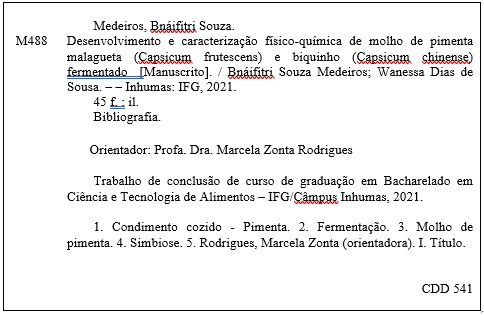
\includegraphics[width=0.8\textwidth]{ficha_catalografica.jpg} \\[1.5cm]
	
	% Texto inferior
	{\small 
		Ficha catalográfica elaborada pela bibliotecária Maria Aparecida Rodrigues de Souza CRB/1-1497 \\[0.5cm]
		Instituto Federal de Educação, Ciência e Tecnologia de Goiás \\[0.5cm]
		Campus Inhumas - Biblioteca Atena
	} \\[1cm]
	
	% Data
	{\small \today}
	
	\vfill % Preenche o espaço restante automaticamente para centralizar
\end{titlepage}



% -----------------------------------------------------------------------------
% TCC AODV-EN -- Huakson Lima e Diogo dos Reis Almeida (IFG Campus Inhumas).
% Este template foi criado para atender às necessidades acadêmicas dos discentes
% do  Instituto Federal de Educação, Ciência e Tecnologia de Goiás (IFG), unindo 
% precisão, padronização e automação no uso do LaTeX.
% -----------------------------------------------------------------------------
% Ativar o deslocamento de datas no início do arquivo

\noindent
\begin{center}
	{\bfseries\normalsize TERMO DE AUTORIZAÇÃO PARA DISPONIBILIZAÇÃO \\ NO REPOSITÓRIO DIGITAL DO IFG - ReDi IFG}
\end{center}

\vspace{0.25cm}

Com base no disposto na Lei Federal nº 9.610/98, AUTORIZO o Instituto Federal de Educação, Ciência e Tecnologia de Goiás, a disponibilizar gratuitamente o documento no Repositório Digital (ReDi IFG), sem ressarcimento de direitos autorais, conforme permissão assinalada abaixo, em formato digital para fins de leitura, download e impressão, a título de divulgação da produção técnico-científica no IFG.

\vspace{0.25cm}

\noindent\textbf{Identificação da Produção Técnico-Científica}
\vspace{0.25cm}

\noindent
\begin{tabular}{p{8,5cm} p{7cm}}
	[ \hspace{0.25cm} ] Tese & [\hspace{0.25cm} ] Artigo Científico \\[0.25cm]
	[ \hspace{0.25cm} ] Dissertação & [ \hspace{0.25cm} ] Capítulo de Livro \\[0.25cm]
	[ \hspace{0.25cm} ] Monografia – Especialização & [ \hspace{0.25cm} ] Livro \\[0.25cm]
	[ \hspace{0.25cm} ] TCC – Graduação & [ \hspace{0.25cm} ] Trabalho Apresentado em Evento \\[0.25cm]
	[ \hspace{0.25cm} ] Produto Técnico e Educacional - Tipo:  & \\[0.25cm]
\end{tabular}

\vspace{0.25cm}

\noindent\textbf{Nome Completo do Autor:} \hspace{8cm} \\[0.5cm]
\textbf{Matrícula:} \hspace{11cm} \\[0.5cm]
\textbf{Título do Trabalho:} \hspace{8.5cm}

\vspace{0.25cm}

\noindent\textbf{Autorização - Marque uma das opções}
\vspace{0.25cm}

\noindent
\begin{tabular}{p{15cm}}
[\hspace{0.25cm} ] Autorizo disponibilizar meu trabalho no Repositório Digital do IFG (acesso aberto).\\[0.25cm]
[\hspace{0.25cm} ] Autorizo disponibilizar meu trabalho no Repositório Digital do IFG somente após a data de \today~(Embargo).\\[0.25cm]
[\hspace{0.25cm} ] Não autorizo disponibilizar meu trabalho no Repositório Digital do IFG (acesso restrito).\\[0.25cm]
\end{tabular}

\vspace{0.25cm}

\noindent Ao indicar a opção 2 ou 3, marque a justificativa:
\vspace{0.25cm}

\noindent
\begin{tabular}{p{15cm}}
	[ \hspace{0.25cm} ] O documento está sujeito a registro de patente. \\[0.25cm]
	[ \hspace{0.25cm} ] O documento poderá vir a ser publicado como livro, capítulo de livro ou artigo. \\[0.25cm]
	[ \hspace{0.25cm} ] Outra justificativa: \\[0.25cm]
\end{tabular}

\vspace{0.25cm}

\noindent\rule{10cm}{0.4pt} \\[0.25cm]
\noindent Assinatura do Autor

\clearpage
% -----------------------------------------------------------------------------
% TCC AODV-EN -- Huakson Lima e Diogo dos Reis Almeida (IFG Campus Inhumas).
% Este template foi criado para atender às necessidades acadêmicas dos discentes
% do  Instituto Federal de Educação, Ciência e Tecnologia de Goiás (IFG), unindo 
% precisão, padronização e automação no uso do LaTeX.
% -----------------------------------------------------------------------------
\noindent
\begin{center}
	{\bfseries\large DECLARAÇÃO DE DISTRIBUIÇÃO NÃO-EXCLUSIVA}
\end{center}

\vspace{1cm}

O(A) referido(a) autor(a) declara que:

\vspace{0.5cm}

\begin{enumerate}[label=\roman*.]
	\item o documento é seu trabalho original, detém os direitos autorais da produção técnico-científica e não infringe os direitos de qualquer outra pessoa ou entidade;
	
	\item obteve autorização de quaisquer materiais inclusos no documento de que não detém os direitos de autoria, para conceder ao Instituto Federal de Educação, Ciência e Tecnologia de Goiás os direitos requeridos e que este material cumpre direitos autorais são de terceiros, estão claramente identificados e reconhecidos no texto ou conteúdo do documento entregue;
	
	\item cumpriu quaisquer obrigações exigidas por contrato ou acordo, caso o documento entregue seja baseado em trabalho financiado ou apoiado por outra instituição que não o Instituto Federal de Educação, Ciência e Tecnologia de Goiás.
\end{enumerate}

\vspace{1cm}

\noindent
\begin{tabular}{p{16cm}}
    Inhumas/Goiás \\[0.1cm]
    Local \\[1cm]
    \today \\[0.1cm]
    Data
\end{tabular}


\vspace{2cm}

\noindent\rule{10cm}{0.4pt} \\[0.5cm]
\noindent Assinatura do Autor e/ou Detentor dos Direitos Autorais

% -----------------------------------------------------------------------------
% Este código foi desenvolvido pelo Prof. Wesley Pacheco Calixto, em 26/11/2024.
% Este template foi criado para atender às necessidades acadêmicas dos discentes
% do  Instituto Federal de Educação, Ciência e Tecnologia de Goiás (IFG), unindo 
% precisão, padronização e automação no uso do LaTeX.
% -----------------------------------------------------------------------------
\begin{titlepage}
	% Insere o texto na parte superior
	\begin{center}
		{\small Documento elaborado pelo coordenador do curso.}
	\end{center}
	
	\vspace{1cm} % Espaço entre o texto e a imagem
	
	% Insere a imagem ajustada para caber na mesma página
	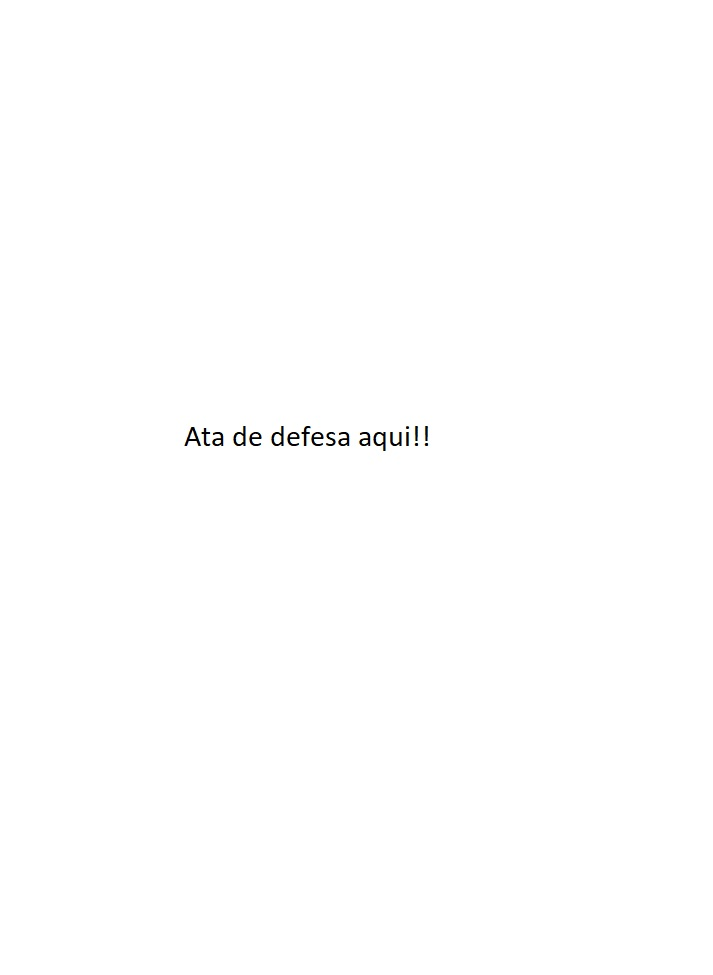
\includegraphics[width=\paperwidth, height=0.9\textheight, keepaspectratio]{ata_defesa.jpg}
	
\end{titlepage}

% -----------------------------------------------------------------------------
% Este código foi desenvolvido pelo Prof. Wesley Pacheco Calixto, em 26/11/2024.
% Este template foi criado para atender às necessidades acadêmicas dos discentes
% do  Instituto Federal de Educação, Ciência e Tecnologia de Goiás (IFG), unindo 
% precisão, padronização e automação no uso do LaTeX.
% -----------------------------------------------------------------------------
\begin{titlepage}
	\begin{center}
		{\bfseries\Large AGRADECIMENTOS} % Título da página centralizado e em destaque
		\vspace{2cm} % Espaçamento entre o título e o texto
	\end{center}
	
	\noindent
Nesta seção, você deve expressar seus agradecimentos às pessoas e instituições que contribuíram para a realização deste trabalho. Podem ser incluídos agradecimentos a Deus, familiares, amigos, orientadores, professores, colegas de curso e demais pessoas ou entidades que prestaram apoio acadêmico, emocional ou material durante o desenvolvimento do TCC.

\hfill \textit{Autor} 
\newline
\newline

	\vspace{2cm} % Espaçamento inferior
\end{titlepage}

% -----------------------------------------------------------------------------
% Conteudo AODV-EN. Template base: Prof. Wesley Pacheco Calixto (IFG).
% -----------------------------------------------------------------------------
\addcontentsline{toc}{section}{Resumo}

\section*{Resumo}

As redes mesh sem fio de baixo custo construídas sobre o protocolo ESP-NOW carecem de
suporte nativo a roteamento multi-hop, o que limita seu alcance e escalabilidade. Este
trabalho propõe, implementa e avalia o AODV-EN, uma adaptação do protocolo Ad-hoc
On-Demand Distance Vector (AODV, RFC 3561) para operação sobre ESP-NOW em módulos ESP32,
contemplando endereçamento por MAC, disseminação de requisições de rota por
\emph{flooding} controlado sobre \emph{broadcast} de enlace, manutenção de rotas com
números de sequência e confirmação fim-a-fim. Adotando o paradigma \emph{Design Science
Research}, o núcleo do protocolo foi implementado em linguagem C como componente
reutilizável e comparado a um algoritmo de referência baseado em \emph{flooding},
medindo-se \emph{Packet Delivery Ratio} (PDR), latência fim-a-fim, \emph{Normalized
Routing Load} (NRL) e consumo energético estimado. No cenário avaliado em hardware (três
ESP32, seis repetições), os dois algoritmos apresentaram confiabilidade equivalente
(PDR de 98,93\% para o AODV-EN e 98,77\% para o \emph{flooding}), com vantagem do AODV-EN
em latência (60,0 ms estáveis contra 62 a 100 ms) e em consumo energético estimado
(aproximadamente 21\% inferior), ao custo de uma carga de controle normalizada de 0,77.
A análise por simulação evidenciou que a desvantagem de ocupação de canal do
\emph{flooding} cresce com a escala da rede, com cruzamento de eficiência em torno de
9 a 11 nós. Conclui-se que o roteamento reativo do AODV-EN é vantajoso à medida que a
rede cresce em tamanho e diâmetro, viabilizando redes mesh padronizadas, de baixo custo
e eficientes em energia sobre ESP-NOW.

\vspace{1cm}

\noindent
\textbf{Palavras-chave:} redes mesh; ESP-NOW; ESP32; AODV; roteamento ad-hoc;
Internet das Coisas.

\clearpage
% -----------------------------------------------------------------------------
% Conteudo AODV-EN. Template base: Prof. Wesley Pacheco Calixto (IFG).
% -----------------------------------------------------------------------------
\addcontentsline{toc}{section}{Abstract}

\section*{Abstract}

Low-cost wireless mesh networks built on top of the ESP-NOW protocol lack native support
for multi-hop routing, which limits their range and scalability. This work proposes,
implements, and evaluates AODV-EN, an adaptation of the Ad-hoc On-Demand Distance Vector
protocol (AODV, RFC 3561) to operate over ESP-NOW on ESP32 modules, featuring MAC-based
addressing, route request dissemination through controlled flooding over link-layer
broadcast, route maintenance with sequence numbers, and end-to-end acknowledgment.
Following the Design Science Research paradigm, the protocol core was implemented in C as
a reusable component and compared against a flooding-based reference algorithm, measuring
Packet Delivery Ratio (PDR), end-to-end latency, Normalized Routing Load (NRL), and
estimated energy consumption. In the hardware scenario C1 (ten ESP32 nodes in a
multi-hop chain of three to four hops, thirty repetitions per algorithm), AODV-EN
delivered 94.1\% of packets versus only 13.9\% for flooding --- a striking gap in the
multi-hop regime, where flooding collapses for lack of a route and retransmission ---
while costing about 20\% fewer transmissions per delivered packet (54.2 versus 68.8). A
second hardware scenario (C3, a dense ten-node mesh, five hops) showed that this advantage
is topology-dependent: in the mesh, path redundancy raises flooding's delivery to 77.8\%,
narrowing --- without eliminating --- AODV-EN's advantage (91.4\%). Simulation analysis
confirmed that the channel-occupancy disadvantage of flooding grows with network scale,
with AODV-EN's efficiency advantage consolidating beyond about eleven nodes. A third hardware scenario (C4, six
nodes), with cyclic failure of an on-path relay, demonstrated the protocol's self-healing:
AODV-EN sustained 70.6\% delivery by rediscovering the route through an alternative relay
after each outage. Regarding estimated energy efficiency,
although AODV-EN's raw aggregate consumption is higher, its energy per successfully
delivered packet is about five times lower than flooding's (0.69 versus 3.75~J/packet),
since routing delivers far more. It is concluded that AODV-EN's reactive routing becomes
advantageous as the network grows in size and diameter, enabling standardized, low-cost
mesh networks over ESP-NOW that are energy-efficient per useful delivery.

\vspace{1cm}

\noindent
\textbf{Keywords:} mesh networks; ESP-NOW; ESP32; AODV; ad-hoc routing;
Internet of Things.


\tableofcontents
\listoffigures
\listoftables

% textos
\mainmatter
\pagenumbering{arabic}
\setcounter{page}{1}

% -----------------------------------------------------------------------------
% Conteudo AODV-EN. Template base: Prof. Wesley Pacheco Calixto (IFG).
% -----------------------------------------------------------------------------
\chapter{INTRODUÇÃO}\label{introduuxe7uxe3o}

No início da década de 1990, Mark Weiser, pesquisador do Xerox Palo Alto
Research Center (PARC), introduziu em seu artigo seminal \emph{The
Computer for the 21st Century} o conceito de Computação Ubíqua, ao
afirmar que as tecnologias mais profundas são aquelas que desaparecem,
integrando-se de forma invisível ao cotidiano humano \cite{weiser1991}.
Essa visão pioneira antecipou um ecossistema composto por centenas de
dispositivos computacionais de baixo custo, baixo consumo energético e
amplamente interconectados por redes sem fio, operando em diferentes
escalas espaciais e comunicando-se de forma transparente entre si e com
o ambiente. Mais de três décadas depois, tal paradigma materializa-se
por meio da Internet das Coisas (\emph{Internet of Things} -- IoT) e das
Redes de Sensores Sem Fio (\emph{Wireless Sensor Networks} -- WSNs),
tecnologias que conectam bilhões de dispositivos embarcados mundialmente
em aplicações que vão desde automação residencial e agricultura de
precisão até monitoramento ambiental e sistemas industriais inteligentes
\cite{priyadarshi2025}.

Nesse contexto, o microcontrolador ESP32, desenvolvido pela Espressif
Systems, destaca-se como uma plataforma versátil e amplamente adotada,
combinando conectividade Wi-Fi e Bluetooth integradas, elevado poder de
processamento e custo acessível, características que o tornam ideal para
prototipagem e implantação de soluções IoT em escala. Entretanto, a
comunicação em redes IoT frequentemente enfrenta desafios relacionados à
cobertura, escalabilidade e resiliência. Topologias centralizadas, como
a estrela, apresentam limitações significativas: a dependência de um
ponto de acesso único constitui um gargalo de desempenho e um ponto
único de falha, comprometendo a robustez do sistema \cite{chaizeng2021}.

Como alternativa, as Redes Mesh Sem Fio (\emph{Wireless Mesh Networks}
-- WMNs) emergem como uma solução promissora, oferecendo características
de auto-organização (\emph{self-configuration}), auto-recuperação
(\emph{self-healing}) e comunicação ponto-a-ponto entre os nós
participantes. Nas redes mesh, a comunicação em múltiplos saltos
(\emph{multi-hop}) permite que pacotes de dados sejam encaminhados
através de nós intermediários até alcançarem seu destino final,
estendendo significativamente o alcance da rede sem a necessidade de
aumentar a potência de transmissão dos dispositivos individuais
\cite{arregui2025}. Essa abordagem possibilita a implantação de redes em
áreas extensas utilizando dispositivos de baixa potência, reduzindo
custos e consumo energético. Em contrapartida, a comunicação multi-hop
introduz desafios adicionais relacionados ao roteamento de pacotes,
gerenciamento de interferência e manutenção da topologia da rede,
exigindo algoritmos especializados para garantir a entrega confiável dos
dados.

Para enfrentar esses desafios, os protocolos de roteamento para redes
ad-hoc podem ser classificados em três categorias principais: proativos,
reativos e híbridos. Os protocolos proativos, como o \emph{Optimized
Link State Routing} (OLSR), mantêm tabelas de roteamento constantemente
atualizadas, oferecendo baixa latência na descoberta de rotas às custas
de maior \emph{overhead} de controle. Os protocolos reativos, como o
\emph{Ad-hoc On-Demand Distance Vector} (AODV), descobrem rotas apenas
quando necessário, reduzindo o tráfego de controle em redes com tráfego
esporádico. Já os protocolos híbridos combinam características de ambas
as abordagens, adaptando-se às diferentes condições da rede
\cite{chaizeng2021}.

Entre os mecanismos de comunicação disponíveis no ecossistema ESP32, o
protocolo ESP-NOW destaca-se como uma alternativa de alto desempenho
para comunicação direta entre dispositivos. O ESP-NOW opera de forma
\emph{connectionless} sobre a camada
de enlace do padrão IEEE 802.11 e permite a troca de mensagens curtas
(até 250 bytes de \emph{payload}) sem a necessidade de estabelecimento
prévio de conexão ou associação a um ponto de acesso Wi-Fi
\cite{becker2025}. Estudos experimentais recentes demonstram as
vantagens do ESP-NOW em relação a outras tecnologias de comunicação sem
fio. \citeonline{becker2025}, em experimentos de campo conduzidos em
ambientes abertos e florestais, reportaram latências médias de 2,8 ms e
\emph{Packet Delivery Ratio} (PDR) superior a 99\% em distâncias de até
55 metros em condições de linha de visada. \citeonline{urazayev2023},
avaliando o protocolo em ambiente interno, constataram que o ESP-NOW
apresenta alcance 15\% superior e consumo energético 30\% inferior
quando comparado a soluções baseadas em Wi-Fi TCP convencional. Essas
características tornam o ESP-NOW especialmente atrativo para aplicações
IoT em ambientes remotos ou alimentados por baterias de capacidade
limitada.

Apesar de suas vantagens, o protocolo apresenta limitações estruturais
que restringem sua aplicabilidade em cenários que demandam redes de
maior escala ou alcance estendido. A primeira limitação refere-se à
ausência de suporte nativo a roteamento multi-hop: o ESP-NOW foi
concebido exclusivamente para comunicações ponto-a-ponto ou em topologia
estrela, não oferecendo mecanismos intrínsecos para encaminhamento de
pacotes através de nós intermediários \cite{becker2025}. A segunda
limitação diz respeito ao número máximo de \emph{peers} simultâneos
suportados: cada dispositivo ESP32 pode manter no máximo 20 \emph{peers}
registrados em sua tabela de pares, o que impõe restrições severas à
escalabilidade da rede. A terceira limitação relaciona-se à ausência de
mecanismo de \emph{broadcast} nativo eficiente, dificultando a
disseminação de mensagens de controle necessárias para protocolos de
descoberta de rotas. Essa lacuna torna-se evidente ao se analisarem
soluções de redes em malha amplamente utilizadas no ecossistema
Espressif, como o ESP-WIFI-MESH e a biblioteca PainlessMesh, que operam
sobre a pilha Wi-Fi convencional (IEEE 802.11). Conforme discutido por
\citeonline{sestak2022}, o uso do Wi-Fi padrão para manutenção da
topologia mesh impõe elevado \emph{overhead} de processamento e consumo
energético, inviabilizando sua aplicação em dispositivos estritamente
alimentados por baterias e comprometendo a principal vantagem
competitiva do ESP-NOW. Trabalhos recentes têm buscado preencher essa
lacuna: \citeonline{cujilema2023} propuseram o algoritmo BRAM-NOW para
criação de redes mesh seguras sobre ESP-NOW, demonstrando latência média
de 75 ms e taxa de perda de pacotes de 9,25\% em ambiente residencial.
Entretanto, tal abordagem não se fundamenta em protocolos de roteamento
padronizados, o que dificulta sua comparação com soluções estabelecidas
na literatura e limita sua extensibilidade.

Diante desse cenário, formula-se a seguinte questão de pesquisa: é
viável adaptar um protocolo de roteamento padronizado e amplamente
validado, como o AODV, para operar sobre o ESP-NOW, contornando suas
restrições de \emph{peers}, ausência de \emph{broadcast} confiável e de
suporte a multi-hop, mantendo desempenho competitivo frente a uma
abordagem de referência baseada em inundação (\emph{flooding})? Como
hipótese central, admite-se que um roteamento reativo sob demanda,
adaptado a essas restrições, é capaz de entregar pacotes em múltiplos
saltos sobre ESP-NOW com taxa de entrega comparável à da inundação
controlada, porém a um custo de controle e de ocupação de canal
significativamente menor à medida que a rede cresce em tamanho e
diâmetro.

Para responder a essa questão, o presente trabalho propõe o
desenvolvimento e a avaliação de um algoritmo de roteamento denominado
AODV-EN (\emph{Ad-hoc On-Demand Distance Vector for ESP-NOW}), uma
adaptação do protocolo AODV, especificado na RFC 3561 \cite{perkins2003}.
A escolha do AODV como protocolo base justifica-se por suas
características de roteamento reativo sob demanda, que minimizam o
tráfego de controle em redes com comunicação intermitente, e por sua
ampla documentação e validação na literatura acadêmica, facilitando
comparações e extensões futuras. As principais adaptações propostas para
adequar o AODV às restrições do ESP-NOW incluem: (i) gerenciamento
dinâmico de \emph{peers} utilizando política LRU (\emph{Least Recently
Used}), com cache configurável de entradas ativas, permitindo que o
protocolo alcance nós em número superior ao do cache ao longo do tempo,
dentro do limite físico de 20 \emph{peers} do ESP-NOW; (ii) disseminação
das mensagens RREQ (\emph{Route Request}) por \emph{flooding} controlado
sobre \emph{broadcast} de enlace do ESP-NOW (FF:FF:FF:FF:FF:FF), com
supressão de duplicatas por cache de identificadores e limite de
propagação (TTL), preservando a semântica clássica do AODV; e (iii)
incorporação de métrica híbrida de roteamento que combina contagem de
saltos (\emph{hop count}) com indicador de qualidade do sinal recebido
(RSSI), possibilitando a seleção de rotas que equilibrem menor distância
lógica e melhor qualidade de enlace.

\section{OBJETIVOS}\label{objetivos}

Esta seção apresenta o objetivo geral e os objetivos específicos que
orientam o desenvolvimento deste trabalho.

\subsection{Objetivo geral}\label{objetivo-geral}

Propor, implementar e avaliar um algoritmo de roteamento multi-hop
baseado no protocolo AODV, adaptado para operação em redes mesh
construídas sobre o protocolo ESP-NOW, considerando as restrições
específicas dessa tecnologia e utilizando hardware de baixo custo.

\subsection{Objetivos específicos}\label{objetivos-especuxedficos}

Para alcançar o objetivo geral, foram definidos os seguintes objetivos
específicos:

\begin{enumerate}
\def\labelenumi{\alph{enumi})}
\tightlist
\item
  Analisar as limitações técnicas do protocolo ESP-NOW para comunicação
  multi-hop, identificando os desafios específicos relacionados ao
  limite de \emph{peers}, ausência de \emph{broadcast} nativo e
  gerenciamento de rotas;
\item
  Projetar as adaptações necessárias ao protocolo AODV para adequá-lo às
  restrições do ESP-NOW, incluindo gerenciamento de \emph{peers} com
  política LRU, \emph{flooding} controlado e métrica híbrida de
  roteamento;
\item
  Implementar um protótipo funcional do algoritmo AODV-EN em módulos
  ESP32, desenvolvendo as estruturas de dados, mensagens de controle e
  mecanismos de descoberta e manutenção de rotas;
\item
  Avaliar o desempenho do algoritmo proposto através de experimentos em
  diferentes topologias de rede, utilizando métricas quantitativas como
  \emph{Packet Delivery Ratio} (PDR), latência fim-a-fim,
  \emph{Normalized Routing Load} (NRL) e consumo energético;
\item
  Comparar os resultados obtidos com trabalhos correlatos da literatura,
  posicionando a contribuição do AODV-EN em relação às soluções
  existentes para redes mesh sobre ESP-NOW e outras tecnologias.
\end{enumerate}

\section{CENÁRIOS DE APLICAÇÃO}\label{cenarios-de-aplicacao}

A motivação para prover roteamento multi-hop padronizado sobre ESP-NOW
torna-se concreta em cenários nos quais a infraestrutura de rede é
ausente, intermitente ou economicamente inviável, mas a comunicação entre
muitos dispositivos de baixo custo e baixo consumo é necessária ao longo
de áreas que excedem o alcance de um único enlace. Quatro classes de
aplicação ilustram a relevância da proposta:

\begin{itemize}
\item \textbf{Agricultura de precisão e monitoramento rural.} Sensores de
  umidade do solo, temperatura e nível de reservatórios distribuídos por
  uma propriedade extensa, sem cobertura de Wi-Fi ou celular, podem
  encaminhar leituras até um concentrador por múltiplos saltos, a custo de
  hardware da ordem de poucos dólares por nó.
\item \textbf{Monitoramento industrial e predial.} Em galpões, plantas
  fabris e edifícios, paredes e estruturas metálicas fragmentam a
  conectividade; uma malha auto-organizável que contorna obstáculos por
  rotas alternativas é mais robusta que enlaces ponto a ponto.
\item \textbf{Redes comunitárias e resposta a desastres.} Em regiões sem
  infraestrutura ou após eventos que a destroem, nós alimentados por
  bateria podem formar rapidamente uma malha temporária para troca de
  mensagens e telemetria, sem depender de pontos de acesso.
\item \textbf{Automação residencial de baixo custo.} Dispositivos
  domésticos (sensores, atuadores) distribuídos por uma casa de vários
  cômodos, onde a atenuação por paredes já exige multi-hop, conforme
  observado no próprio cenário experimental deste trabalho.
\end{itemize}

Em todos esses contextos, a adoção de um protocolo \emph{padronizado}
(AODV, RFC 3561), em vez de uma solução \emph{ad hoc} proprietária,
favorece a interoperabilidade, a reprodutibilidade e a manutenção de longo
prazo --- diferencial central da proposta.

\section{ESTRUTURA DO TRABALHO}\label{estrutura-do-trabalho}

Além desta introdução, este trabalho está organizado em mais cinco
capítulos. O Capítulo~\ref{cap:referencial} apresenta o referencial
teórico, abordando as redes de sensores sem fio e redes mesh, o
protocolo ESP-NOW e suas limitações, os protocolos de roteamento ad-hoc
e o protocolo AODV, o algoritmo de inundação utilizado como referência e
as métricas de avaliação de desempenho. O Capítulo~\ref{cap:metodologia}
descreve a metodologia adotada, fundamentada na \emph{Design Science
Research}, detalhando os cenários experimentais, os parâmetros de
configuração e o procedimento de coleta e análise dos dados. O
Capítulo~\ref{cap:implementacao} apresenta o projeto e a implementação
do AODV-EN, incluindo a arquitetura do firmware, as estruturas de dados,
o formato das mensagens e as adaptações propostas. O
Capítulo~\ref{cap:resultados} reporta e discute os resultados obtidos na
avaliação experimental em \emph{hardware} e em simulação, comparando o
AODV-EN com o algoritmo de referência e com a literatura correlata. Por
fim, o Capítulo~\ref{cap:conclusao} apresenta as conclusões, as
limitações do estudo e as propostas de trabalhos futuros.

% -----------------------------------------------------------------------------
% Conteudo AODV-EN. Template base: Prof. Wesley Pacheco Calixto (IFG).
% -----------------------------------------------------------------------------
\chapter{REFERENCIAL TEÓRICO}\label{cap:referencial}\label{referencial-teuxf3rico}

Este capítulo apresenta os fundamentos teóricos que embasam o
desenvolvimento da pesquisa. Inicialmente, são discutidos os conceitos
de Internet das Coisas e de Redes de Sensores Sem Fio, situando o
contexto tecnológico do estudo. Em seguida, são apresentadas as
características do microcontrolador ESP32 e do protocolo ESP-NOW,
utilizados na implementação do artefato. Posteriormente, abordam-se os
conceitos de redes mesh e a classificação dos protocolos de roteamento
ad-hoc. Por fim, é analisado o protocolo AODV, que fundamenta a
adaptação proposta e o desenvolvimento do protocolo AODV-EN.

\section{Internet das Coisas e Redes de Sensores Sem
Fio}\label{internet-das-coisas-e-redes-de-sensores-sem-fio}

A Internet das Coisas (\emph{Internet of Things} -- IoT) representa um
paradigma tecnológico no qual objetos físicos dotados de capacidade
computacional, sensores e conectividade de rede integram-se ao ambiente
de forma ubíqua, coletando e compartilhando dados sem intervenção humana
direta \cite{priyadarshi2025}. Essa visão, antecipada por Mark Weiser em
1991 sob o conceito de Computação Ubíqua \cite{weiser1991}, materializa-se atualmente em
bilhões de dispositivos conectados mundialmente, permeando setores como
saúde, agricultura, indústria, cidades inteligentes e automação
residencial. As Redes de Sensores Sem Fio (\emph{Wireless Sensor
Networks} -- WSNs) constituem uma das principais infraestruturas para
implementação de aplicações IoT. Uma WSN é composta por um conjunto de
nós sensores distribuídos espacialmente, capazes de monitorar fenômenos
físicos ou ambientais, como temperatura, umidade, pressão, movimento ou
luminosidade, e transmitir os dados coletados por meio de enlaces sem fio
até uma estação base ou gateway \cite{chaizeng2021}. Os nós sensores são
tipicamente dispositivos de recursos limitados, com restrições de
processamento, memória, energia e largura de banda de comunicação. O
projeto de WSNs deve considerar um conjunto de requisitos críticos que
influenciam diretamente a viabilidade e eficácia das aplicações. O
Quadro~\ref{quadro:req-wsn} sintetiza os principais requisitos e suas implicações para o
projeto de redes de sensores.

{\def\LTcaptype{quadro}
\begin{longtable}[]{@{}
  >{\centering\arraybackslash}p{(\linewidth - 2\tabcolsep) * \real{0.5000}}
  >{\centering\arraybackslash}p{(\linewidth - 2\tabcolsep) * \real{0.5000}}@{}}
\caption{Requisitos críticos para projeto de Redes de Sensores Sem Fio}\label{quadro:req-wsn}\\
\toprule\noalign{}
\begin{minipage}[b]{\linewidth}\centering
Requisito
\end{minipage} & \begin{minipage}[b]{\linewidth}\centering
Descrição e Implicações
\end{minipage} \\
\midrule\noalign{}
\endhead
\bottomrule\noalign{}
\endlastfoot
Baixo custo & Implantações em larga escala requerem dispositivos
economicamente acessíveis. O custo por nó deve permitir a instalação de
dezenas a centenas de dispositivos sem inviabilizar o projeto. \\
Baixo consumo energético & Muitas aplicações exigem operação por meses
ou anos com baterias de capacidade limitada. O consumo deve ser
minimizado em todos os subsistemas: processamento, comunicação e
sensoriamento. \\
Confiabilidade & A rede deve garantir a entrega dos dados coletados
mesmo em condições adversas, como interferência eletromagnética,
obstáculos físicos ou falha de nós individuais. \\
Escalabilidade & A arquitetura deve suportar o crescimento do número de
nós sem degradação significativa de desempenho ou necessidade de
reconfiguração manual. \\
Auto-organização & Os nós devem ser capazes de estabelecer e manter a
topologia da rede de forma autônoma, adaptando-se a mudanças no ambiente
ou na composição da rede. \\
\end{longtable}
}

Fonte: Adaptado de \citeonline{priyadarshi2025} e \citeonline{chaizeng2021}.

A comunicação sem fio é o componente de maior consumo energético em um
nó sensor típico, podendo representar até 70\% do consumo total do
dispositivo \cite{priyadarshi2025}. Dessa forma, a escolha do protocolo
de comunicação e a estratégia de roteamento adotada impactam diretamente
a vida útil da rede. Protocolos que minimizam o número de transmissões,
utilizam modos de baixo consumo durante períodos de inatividade e
otimizam o tamanho das mensagens de controle contribuem
significativamente para a extensão da autonomia dos dispositivos.

\section{O Microcontrolador ESP32}\label{o-microcontrolador-esp32}

O ESP32 é um \emph{System-on-Chip} (SoC) desenvolvido pela Espressif
Systems, projetado para aplicações de Internet das Coisas que demandam
conectividade sem fio integrada, desempenho computacional elevado e
eficiência energética. Desde seu lançamento em 2016, o ESP32 tornou-se
uma das plataformas mais populares para prototipagem e desenvolvimento
de soluções IoT, sendo utilizado tanto em projetos acadêmicos quanto em
produtos comerciais \cite{becker2025}. A arquitetura do ESP32 baseia-se
em um processador dual-core Xtensa LX6, operando em frequências de até
240 MHz, complementado por coprocessador de ultra-baixo consumo (ULP),
memória SRAM de 520 KB e suporte a memória flash externa de até 16 MB. O
SoC integra interfaces Wi-Fi 802.11 b/g/n e Bluetooth 4.2 (incluindo
BLE), além de um amplo conjunto de periféricos como conversores
analógico-digitais (ADC), conversores digital-analógicos (DAC),
interfaces SPI, I²C, I²S, UART, PWM, sensores de toque capacitivo e
sensor de efeito Hall. O Quadro~\ref{quad:esp32-specs} sintetiza as principais especificações técnicas do dispositivo.

O Quadro~\ref{quadro:esp32-specs} resume as principais especificações técnicas do ESP32.

{\def\LTcaptype{quadro}
\begin{longtable}[]{@{}cl@{}}
\caption{Especificações técnicas do microcontrolador ESP32}\label{quadro:esp32-specs}\\
\toprule\noalign{}
Característica & Especificação \\
\midrule\noalign{}
\endhead
\bottomrule\noalign{}
\endlastfoot
Processador & Dual-core Xtensa LX6, até 240 MHz \\
Coprocessador & ULP (Ultra Low Power) para operação em deep sleep \\
Memória SRAM & 520 KB \\
Flash externa & Até 16 MB (tipicamente 4 MB em módulos DevKit) \\
Conectividade Wi-Fi & IEEE 802.11 b/g/n, 2.4 GHz, até 150 Mbps \\
Conectividade Bluetooth & Bluetooth 4.2 BR/EDR e BLE \\
Tensão de operação & 3.0 V -- 3.6 V (típico 3.3 V) \\
GPIOs & 34 pinos programáveis \\
Interfaces & SPI, I²C, I²S, UART, PWM, ADC (12-bit), DAC (8-bit) \\
\end{longtable}
}

Fonte: \citeonline{espressif2024}.

Uma característica diferencial do ESP32 para aplicações IoT é seu
suporte a múltiplos modos de operação com diferentes perfis de consumo
energético. O Quadro~\ref{quadro:esp32-energia} apresenta os modos de energia disponíveis e seus
respectivos consumos típicos, conforme especificado no \emph{datasheet}
do fabricante.

{\def\LTcaptype{quadro}
\begin{longtable}[]{@{}
  >{\raggedright\arraybackslash}p{(\linewidth - 4\tabcolsep) * \real{0.3333}}
  >{\raggedright\arraybackslash}p{(\linewidth - 4\tabcolsep) * \real{0.3333}}
  >{\raggedright\arraybackslash}p{(\linewidth - 4\tabcolsep) * \real{0.3333}}@{}}
\caption{Modos de operação e consumo energético do ESP32}\label{quadro:esp32-energia}\\
\toprule\noalign{}
\begin{minipage}[b]{\linewidth}\raggedright
Modo de Operação
\end{minipage} & \begin{minipage}[b]{\linewidth}\raggedright
Consumo Típico
\end{minipage} & \begin{minipage}[b]{\linewidth}\raggedright
Descrição
\end{minipage} \\
\midrule\noalign{}
\endhead
\bottomrule\noalign{}
\endlastfoot
Active (Wi-Fi TX) & 160 -- 260 mA & Transmissão ativa de dados via
Wi-Fi \\
Active (CPU @ 240 MHz) & 30 -- 68 mA & CPU operando em máxima
frequência, rádio desligado \\
Active (CPU @ 80 MHz) & 20 -- 25 mA & CPU operando em frequência
reduzida, rádio desligado \\
Modem Sleep & 3 -- 20 mA & CPU ativa, rádio Wi-Fi/BT desligado \\
Light Sleep & 0.8 mA & CPU pausada, RAM preservada, despertar rápido
(\textless1 ms) \\
Deep Sleep & 10 -- 150 µA & CPU desligada, apenas RTC ativo, despertar
por timer ou GPIO \\
Hibernation & 5 µA & Apenas RTC timer ativo, memória não preservada \\
\end{longtable}
}

Fonte: \citeonline{espressif2024}.

A disponibilidade de módulos de desenvolvimento (DevKit) a preços
acessíveis, tipicamente entre R\$ 25,00 e R\$ 40,00 no mercado
brasileiro em 2024, democratiza o acesso à tecnologia e viabiliza a construção
de redes de sensores com dezenas de nós a custos compatíveis com
aplicações em países em desenvolvimento.

\section{O Protocolo ESP-NOW}\label{o-protocolo-esp-now}

O ESP-NOW é um protocolo de comunicação sem fio proprietário
desenvolvido pela Espressif Systems, projetado para permitir a troca
direta de mensagens curtas entre dispositivos ESP32 e ESP8266 sem a
necessidade de estabelecimento prévio de conexão Wi-Fi ou associação a
um ponto de acesso. O protocolo opera na camada de enlace do padrão IEEE
802.11, utilizando \emph{action frames} do tipo \emph{vendor-specific}
para transmissão de dados \cite{becker2025}.

\subsection{Características
técnicas}\label{caracteruxedsticas-tuxe9cnicas}

O ESP-NOW opera na frequência de 2.4 GHz, com taxa de transmissão de 1
Mbit/s e largura de banda de canal de 20 MHz. O protocolo implementa um
mecanismo de acesso ao meio baseado em CSMA (\emph{Carrier Sense
Multiple Access}) do tipo \emph{p-persistent}, com \emph{slots}
temporais de aproximadamente 481 µs. O suporte a retransmissões
automáticas permite até 31 tentativas por pacote em caso de falha na
entrega, aumentando a confiabilidade da comunicação \cite{becker2025}.
Cada mensagem ESP-NOW pode transportar até 250 bytes de \emph{payload}
útil, com um \emph{overhead} de cabeçalho de aproximadamente 43 bytes. O
protocolo suporta criptografia opcional utilizando o algoritmo AES-128
no modo CCMP, permitindo comunicação segura quando necessário. A
identificação dos dispositivos é realizada através de seus endereços MAC
de 6 bytes. O Quadro~\ref{quad:espnow-specs} resume as características técnicas do protocolo.

O Quadro~\ref{quadro:espnow-carac} sintetiza as principais características técnicas do ESP-NOW.

{\def\LTcaptype{quadro}
\begin{longtable}[]{@{}
  >{\centering\arraybackslash}p{(\linewidth - 2\tabcolsep) * \real{0.5000}}
  >{\centering\arraybackslash}p{(\linewidth - 2\tabcolsep) * \real{0.5000}}@{}}
\caption{Características técnicas do protocolo ESP-NOW}\label{quadro:espnow-carac}\\
\toprule\noalign{}
\begin{minipage}[b]{\linewidth}\centering
Parâmetro
\end{minipage} & \begin{minipage}[b]{\linewidth}\centering
Valor
\end{minipage} \\
\midrule\noalign{}
\endhead
\bottomrule\noalign{}
\endlastfoot
Padrão base & IEEE 802.11 b/g/n (\emph{action frames} vendor-specific) \\
Frequência de operação & 2.4 GHz (canais 1-14) \\
Taxa de transmissão & 1 Mbit/s \\
Payload máximo & 250 bytes \\
Overhead de cabeçalho & \textasciitilde43 bytes \\
Mecanismo de acesso ao meio & CSMA p-persistent (slot \textasciitilde481
µs) \\
Retransmissões automáticas & Até 31 tentativas por pacote \\
Criptografia & AES-128 CCMP (opcional) \\
Número máximo de peers & 20 peers no total, dos quais até 6 com criptografia habilitada \cite{espressif2024} \\
\end{longtable}
}

Fonte: \citeonline{becker2025}; \citeonline{espressif2024}.

\subsection{Desempenho e alcance}\label{desempenho-e-alcance}

Estudos experimentais recentes fornecem caracterização detalhada do
desempenho do ESP-NOW em diferentes condições. \citeonline{becker2025},
em experimentos de campo conduzidos em 246 posições distintas em
ambientes abertos (fazenda) e florestais, reportaram latência base de
transmissão entre 2.700 e 2.800 µs (aproximadamente 2,8 ms), podendo
alcançar até 60 ms em cenários com múltiplas retransmissões. Em termos
de confiabilidade, foi observado \emph{Packet Delivery Ratio} (PDR)
superior a 99\% em distâncias de até 55 metros em linha de visada, com
alcance máximo de aproximadamente 70 metros antes da perda total de
conectividade. Em ambiente interno, \citeonline{urazayev2023} avaliaram
o desempenho do ESP-NOW considerando a presença de paredes e obstáculos.
Os resultados demonstraram que o ESP-NOW apresenta alcance interno de 15
a 90 metros dependendo das condições, com PDR 15\% superior e consumo
energético 30\% inferior quando comparado a soluções baseadas em Wi-Fi
TCP convencional. Os autores destacam que fatores ambientais como
reflexões e obstáculos afetam significativamente o desempenho, e que
pequenas variações na posição do receptor podem causar grandes
alterações na qualidade do enlace.

\subsection{Limitações para comunicação
multi-hop}\label{limitauxe7uxf5es-para-comunicauxe7uxe3o-multi-hop}

Apesar de suas vantagens, o ESP-NOW apresenta limitações estruturais que
restringem sua aplicação direta em redes de maior escala. A primeira e
mais significativa limitação é a ausência de suporte nativo a roteamento
em múltiplos saltos (\emph{multi-hop}), isto é, ao encaminhamento de
pacotes por nós intermediários até um destino fora do alcance direto. O
protocolo foi concebido exclusivamente para comunicações
ponto-a-ponto ou em topologia estrela, não oferecendo mecanismos para
esse encaminhamento \cite{becker2025}. A segunda limitação refere-se ao número máximo de
\emph{peers} simultâneos: cada dispositivo ESP32 suporta no máximo
20 \emph{peers} registrados na tabela de pares, sendo que apenas 6
desses podem ter criptografia AES-128 habilitada individualmente
\cite{espressif2024}. Essa restrição, imposta por limitações de memória
do hardware, impede a escalabilidade direta da rede e exige estratégias
de gerenciamento dinâmico de \emph{peers} para contorná-la. A terceira limitação relaciona-se à
ausência de mecanismo de \emph{broadcast} nativo eficiente. Embora seja
possível enviar mensagens para o endereço de \emph{broadcast}
(FF:FF:FF:FF:FF:FF), essa abordagem não oferece confirmação de entrega e
apresenta menor confiabilidade, dificultando sua utilização para
disseminação de mensagens de controle em protocolos de descoberta de
rotas.

\section{Redes Mesh e Protocolos de Roteamento
Ad-Hoc}\label{redes-mesh-e-protocolos-de-roteamento-ad-hoc}

\subsection{Conceitos fundamentais de redes
mesh}\label{conceitos-fundamentais-de-redes-mesh}

As Redes Mesh Sem Fio (\emph{Wireless Mesh Networks} -- WMNs) constituem
uma arquitetura de rede descentralizada na qual cada nó pode funcionar
simultaneamente como origem, destino e roteador de dados, estabelecendo
múltiplos caminhos de comunicação entre os participantes
\cite{chaizeng2021}. Diferentemente das topologias centralizadas, como a
estrela, onde todos os nós dependem de um ponto de acesso único, as
redes mesh distribuem a responsabilidade de encaminhamento entre todos
os participantes, eliminando pontos únicos de falha e aumentando a
resiliência do sistema. A comunicação em múltiplos saltos
(\emph{multi-hop}) é uma característica fundamental das redes mesh:
quando o destino está fora do alcance direto de transmissão do nó de
origem, pacotes de dados são encaminhados através de nós intermediários
que atuam como \emph{relays}. Essa abordagem permite estender
significativamente o alcance efetivo da rede sem aumentar a potência de
transmissão individual dos dispositivos, característica particularmente
valiosa para redes de sensores alimentadas por bateria. As WMNs podem
ser classificadas em três categorias principais conforme sua
arquitetura: (i) \emph{Infrastructure WMN}, onde roteadores mesh formam
a infraestrutura de backbone da rede; (ii) \emph{Client WMN}, onde os
próprios dispositivos clientes participam do roteamento; e (iii)
\emph{Hybrid WMN}, que combina características de ambas as abordagens.
Para redes de sensores com ESP32, a arquitetura \emph{Client WMN} é
tipicamente mais adequada, pois todos os nós possuem capacidade
computacional similar e podem contribuir para o roteamento
\cite{chaizeng2021}.

\subsection{Classificação dos protocolos de
roteamento}\label{classificauxe7uxe3o-dos-protocolos-de-roteamento}

Os protocolos de roteamento para redes ad-hoc e mesh podem ser
classificados em três categorias principais conforme sua estratégia de
descoberta e manutenção de rotas: proativos (\emph{table-driven}),
reativos (\emph{on-demand}) e híbridos. Os protocolos proativos, como o
\emph{Optimized Link State Routing} (OLSR) e o
\emph{Destination-Sequenced Distance-Vector} (DSDV), mantêm tabelas de
roteamento constantemente atualizadas através da troca periódica de
informações de topologia entre todos os nós da rede. Essa abordagem
oferece baixa latência na descoberta de rotas --- uma vez que a
informação já está disponível quando necessária --- mas impõe
\emph{overhead} de controle constante, mesmo quando não há tráfego de
dados, o que pode ser problemático para redes de sensores com recursos
energéticos limitados. Os protocolos reativos, como o \emph{Ad-hoc
On-Demand Distance Vector} (AODV) e o \emph{Dynamic Source Routing}
(DSR), descobrem rotas apenas quando há necessidade efetiva de
comunicação. Quando um nó precisa enviar dados para um destino
desconhecido, inicia um processo de descoberta de rota através da
disseminação de mensagens de requisição pela rede. Essa abordagem
elimina o \emph{overhead} de manutenção em períodos de inatividade,
sendo mais adequada para redes com padrões de tráfego esporádicos ou
imprevisíveis, características comuns em aplicações de sensoriamento. Os
protocolos híbridos, como o \emph{Zone Routing Protocol} (ZRP), combinam
características de ambas as abordagens: utilizam roteamento proativo
dentro de zonas locais e roteamento reativo para comunicação entre
zonas. Essa estratégia busca balancear as vantagens de ambas as
abordagens, mas introduz complexidade adicional na implementação. O Quadro~\ref{quad:protocolos-comparativo} sintetiza o comparativo entre as três categorias.

O Quadro~\ref{quadro:comp-protocolos} apresenta um comparativo entre as categorias de protocolos de roteamento ad-hoc.

{\def\LTcaptype{quadro}
\begin{longtable}[]{@{}
  >{\raggedright\arraybackslash}p{(\linewidth - 6\tabcolsep) * \real{0.2500}}
  >{\raggedright\arraybackslash}p{(\linewidth - 6\tabcolsep) * \real{0.2500}}
  >{\raggedright\arraybackslash}p{(\linewidth - 6\tabcolsep) * \real{0.2500}}
  >{\raggedright\arraybackslash}p{(\linewidth - 6\tabcolsep) * \real{0.2500}}@{}}
\caption{Comparativo entre categorias de protocolos de roteamento ad-hoc}\label{quadro:comp-protocolos}\\
\toprule\noalign{}
\begin{minipage}[b]{\linewidth}\raggedright
Característica
\end{minipage} & \begin{minipage}[b]{\linewidth}\raggedright
Proativo
\end{minipage} & \begin{minipage}[b]{\linewidth}\raggedright
Reativo
\end{minipage} & \begin{minipage}[b]{\linewidth}\raggedright
Híbrido
\end{minipage} \\
\midrule\noalign{}
\endhead
\bottomrule\noalign{}
\endlastfoot
Exemplos & OLSR, DSDV & AODV, DSR & ZRP \\
Descoberta de rotas & Antecipada (sempre) & Sob demanda & Combinada \\
Latência inicial & Baixa & Alta (descoberta) & Média \\
Overhead de controle & Constante (alto) & Variável (baixo) & Moderado \\
Uso de memória & Alto & Baixo/médio & Médio \\
Adequação para WSNs & Limitada & Boa & Moderada \\
\end{longtable}
}

Fonte: Adaptado de \citeonline{chaizeng2021} e \citeonline{priyadarshi2025}.

\subsection{Soluções existentes de mesh para
ESP32}\label{soluuxe7uxf5es-existentes-de-mesh-para-esp32}

O ecossistema ESP32 oferece algumas soluções de rede mesh, cada uma com
características distintas. O ESP-WIFI-MESH (também conhecido como
ESP-MDF) é a solução oficial da Espressif, implementando uma arquitetura
de árvore auto-organizada sobre a pilha Wi-Fi convencional. Embora
ofereça recursos avançados de gerenciamento de rede, o ESP-WIFI-MESH
impõe consumo energético elevado devido à utilização contínua do rádio
Wi-Fi para manutenção da topologia \cite{sestak2022}. A biblioteca
PainlessMesh, desenvolvida pela comunidade open-source, oferece uma
alternativa simplificada para criação de redes mesh com ESP32 e ESP8266.
Similar ao ESP-WIFI-MESH, a PainlessMesh opera sobre a pilha Wi-Fi,
herdando as mesmas limitações de consumo energético. Conforme observado
por \citeonline{sestak2022}, o uso do Wi-Fi padrão para manutenção da
topologia mesh resulta em \emph{overhead} significativo de processamento
e energia, comprometendo a aplicabilidade dessas soluções em
dispositivos alimentados por baterias. Abordagens alternativas têm
explorado a construção de redes mesh diretamente sobre o ESP-NOW.
\citeonline{cujilema2023} propuseram o algoritmo BRAM-NOW para criação
de redes mesh seguras, demonstrando latência média de 75 ms e taxa de
perda de pacotes de 9,25\% em ambiente residencial. Entretanto, essa
abordagem não se fundamenta em protocolos de roteamento padronizados,
limitando sua comparabilidade com outras soluções e dificultando
extensões futuras.

\section{O Protocolo AODV}\label{o-protocolo-aodv}

O \emph{Ad-hoc On-Demand Distance Vector} (AODV) é um protocolo de
roteamento reativo especificado na RFC 3561 \cite{perkins2003},
projetado para redes ad-hoc móveis (MANETs) com populações de dezenas a
milhares de nós. O protocolo oferece rápida adaptação a condições
dinâmicas de enlace, baixo \emph{overhead} de processamento e memória, e
utilização eficiente da rede, características que o tornam adequado para
adaptação em redes de sensores com recursos limitados.

\subsection{Mensagens de controle}\label{mensagens-de-controle}

O AODV define quatro tipos de mensagens de controle para descoberta e
manutenção de rotas: a) RREQ (\emph{Route Request}): mensagem de
requisição de rota, disseminada por \emph{broadcast} quando um nó
precisa descobrir um caminho para um destino desconhecido. Contém:
endereço IP de origem, número de sequência de origem, endereço IP de
destino, último número de sequência conhecido do destino, identificador
único da requisição (RREQ ID) e contador de saltos; b) RREP (\emph{Route
Reply}): mensagem de resposta, enviada em unicast de volta à origem
quando o destino ou um nó intermediário com rota válida recebe um RREQ.
Contém: endereço IP de destino, número de sequência de destino, endereço
IP de origem, contador de saltos e tempo de vida da rota; c) RERR
(\emph{Route Error}): mensagem de erro de rota, enviada quando uma
quebra de enlace é detectada. Notifica os nós afetados sobre destinos
que se tornaram inalcançáveis através do enlace interrompido; d)
RREP-ACK (\emph{Route Reply Acknowledgment}): mensagem de confirmação
opcional, utilizada para detectar enlaces unidirecionais quando
necessário.

\subsection{Processo de descoberta de
rotas}\label{processo-de-descoberta-de-rotas}

Quando um nó de origem necessita enviar dados para um destino para o
qual não possui rota válida em sua tabela de roteamento, inicia o
processo de descoberta de rota através da difusão de uma mensagem RREQ.
Antes da transmissão, o nó incrementa seu próprio número de sequência e
armazena o par (endereço de origem, RREQ ID) em um buffer temporal para
evitar reprocessamento de requisições duplicadas. Ao receber um RREQ,
cada nó intermediário: (i) cria ou atualiza uma entrada de rota reversa
para a origem; (ii) incrementa o contador de saltos; (iii) verifica se é
o destino ou se possui rota válida para o destino com número de
sequência adequado; (iv) caso positivo, gera e envia um RREP em unicast;
caso negativo, retransmite o RREQ para seus vizinhos (exceto aquele de
quem recebeu). A mensagem RREP é transmitida em unicast através do
caminho reverso estabelecido durante a propagação do RREQ. À medida que
o RREP percorre esse caminho, cada nó intermediário cria ou atualiza uma
entrada de rota direta para o destino, estabelecendo o próximo salto
(\emph{next hop}) como o vizinho de quem recebeu o RREP. Quando o RREP
alcança a origem, a rota bidirecional está estabelecida e a transmissão
de dados pode iniciar.

\subsection{Números de sequência e prevenção de
loops}\label{nuxfameros-de-sequuxeancia-e-prevenuxe7uxe3o-de-loops}

Uma característica distintiva do AODV é a utilização de números de
sequência de destino para garantir a ausência de loops de roteamento
(\emph{loop freedom}). Cada nó mantém seu próprio número de sequência,
incrementando-o antes de originar uma nova requisição de rota ou
resposta. Os números de sequência permitem distinguir informações de
roteamento atualizadas de informações obsoletas: entre duas rotas para
um mesmo destino, é sempre selecionada aquela com maior número de
sequência; em caso de empate, seleciona-se a rota com menor número de
saltos \cite{perkins2003}.

\subsection{Manutenção de rotas e tratamento de
falhas}\label{manutenuxe7uxe3o-de-rotas-e-tratamento-de-falhas}

O AODV monitora a conectividade com os próximos saltos das rotas ativas
através de dois mecanismos complementares: (i) mensagens HELLO
periódicas, que são RREPs com TTL=1 enviadas a cada HELLO\_INTERVAL
(tipicamente 1 segundo); e (ii) detecção de falha de enlace na camada de
enlace, quando disponível (por exemplo, ausência de ACK em transmissões
IEEE 802.11). Quando uma quebra de enlace é detectada, o nó que
identifica a falha invalida todas as rotas que utilizam o enlace
interrompido e gera uma mensagem RERR listando os destinos afetados. A
mensagem RERR é propagada para os precursores --- nós que utilizam o
remetente como próximo salto para os destinos afetados --- permitindo
que invalidem suas respectivas entradas de rota. Opcionalmente, o nó que
detecta a falha pode tentar reparo local da rota antes de propagar o
RERR.

\subsection{Parâmetros de
configuração}\label{paruxe2metros-de-configurauxe7uxe3o}

A RFC 3561 define valores padrão para diversos parâmetros configuráveis
que influenciam o comportamento e desempenho do protocolo. O Quadro~\ref{quadro:aodv-params}
apresenta os principais parâmetros e seus valores padrão, que podem ser
ajustados conforme as características específicas da rede.

{\def\LTcaptype{quadro}
\begin{longtable}[]{@{}lll@{}}
\caption{Parâmetros de configuração do AODV (RFC 3561)}\label{quadro:aodv-params}\\
\toprule\noalign{}
Parâmetro & Valor Padrão & Descrição \\
\midrule\noalign{}
\endhead
\bottomrule\noalign{}
\endlastfoot
ACTIVE\_ROUTE\_TIMEOUT & 3.000 ms & Tempo de vida de rota ativa \\
HELLO\_INTERVAL & 1.000 ms & Intervalo entre mensagens HELLO \\
ALLOWED\_HELLO\_LOSS & 2 & Perdas de HELLO antes de assumir falha \\
NET\_DIAMETER & 35 & Número máximo de saltos na rede \\
NODE\_TRAVERSAL\_TIME & 40 ms & Tempo estimado de travessia por nó \\
RREQ\_RETRIES & 2 & Tentativas de descoberta de rota \\
RREQ\_RATELIMIT & 10 & Máximo de RREQs por segundo \\
TTL\_START & 1 & TTL inicial para expanding ring search \\
TTL\_INCREMENT & 2 & Incremento de TTL a cada tentativa \\
TTL\_THRESHOLD & 7 & TTL máximo antes de usar NET\_DIAMETER \\
\end{longtable}
}

Fonte: RFC 3561 \cite{perkins2003}.

% -----------------------------------------------------------------------------
% Conteudo AODV-EN. Template base: Prof. Wesley Pacheco Calixto (IFG).
% -----------------------------------------------------------------------------
\chapter{METODOLOGIA}\label{metodologia}

Este capítulo apresenta a metodologia adotada para o desenvolvimento e
avaliação do algoritmo AODV-EN. Inicialmente, realiza-se a
caracterização da pesquisa quanto à sua natureza, abordagem e
procedimentos técnicos. Em seguida, apresenta-se o Design Science
Research (DSR) como paradigma metodológico, justificando sua adequação
ao problema investigado. Na sequência, detalham-se as fases do trabalho
mapeadas às etapas da DSR, o planejamento experimental, as métricas de
avaliação e o algoritmo de referência utilizado para comparação. Por
fim, são descritos os procedimentos de coleta, organização e análise dos
dados experimentais.

\section{Caracterização da
Pesquisa}\label{caracterizauxe7uxe3o-da-pesquisa}

Quanto à sua natureza, esta pesquisa classifica-se como aplicada, pois
visa desenvolver uma solução prática para um problema concreto: a
ausência de suporte nativo a roteamento multi-hop no protocolo ESP-NOW.
Diferentemente da pesquisa básica, que busca ampliar o conhecimento
teórico sem preocupação imediata com aplicação, a pesquisa aplicada
objetiva gerar conhecimento para aplicação prática dirigida à solução de
problemas específicos (GIL, 2017). Quanto aos procedimentos técnicos, a
pesquisa é caracterizada como experimental, uma vez que envolve a
implementação de um protótipo funcional (o algoritmo AODV-EN) e a
realização de testes controlados em ambiente de laboratório. A
experimentação permite manipular variáveis independentes (topologia da
rede, número de nós, padrões de tráfego) e observar seus efeitos sobre
variáveis dependentes (taxa de entrega, latência, consumo energético),
estabelecendo relações de causa e efeito. Quanto à abordagem do
problema, a pesquisa é predominantemente quantitativa, fundamentando-se
na coleta e análise de dados numéricos obtidos através de medições
sistemáticas durante os experimentos. As métricas de desempenho ---
Packet Delivery Ratio (PDR), latência fim-a-fim, Normalized Routing Load
(NRL) e consumo energético --- são quantificadas e submetidas à análise
estatística para validação das hipóteses formuladas.

\section{Design Science Research}\label{design-science-research}

Além da caracterização quanto à natureza, abordagem e procedimentos
técnicos, a pesquisa adota o Design Science Research (DSR) como
paradigma metodológico central para orientar o desenvolvimento e a
avaliação do artefato proposto. A escolha dessa abordagem decorre do
fato de o trabalho não se limitar à análise teórica de um fenômeno, mas
envolver a concepção, implementação e avaliação de uma solução
computacional para um problema prático: a ausência de suporte nativo a
roteamento multi-hop no protocolo ESP-NOW. Nesse contexto, o algoritmo
AODV-EN é compreendido como um artefato computacional, pois materializa
uma proposta de solução por meio de um método de roteamento adaptado às
restrições técnicas do ESP-NOW e implementado em módulos ESP32. Dessa
forma, a DSR fornece uma estrutura adequada para organizar o ciclo de
identificação do problema, definição dos objetivos da solução,
desenvolvimento do artefato, demonstração, avaliação e comunicação dos
resultados.

\subsection{Fundamentos da DSR}\label{fundamentos-da-dsr}

O Design Science Research (DSR) é um paradigma de pesquisa orientado à
criação e avaliação de artefatos inovadores destinados a resolver
problemas práticos. Conforme \citeonline{hevner2004}, enquanto as
ciências naturais buscam descrever e explicar fenômenos existentes, as
ciências do design concentram-se em como as coisas deveriam ser para
atingir determinados objetivos. O propósito do design é, nas palavras de
\citeonline{simon1996}, ``transformar situações existentes em situações
preferidas''. Um artefato, no contexto da DSR, pode assumir diferentes
formas: construtos (vocabulário e símbolos), modelos (abstrações e
representações), métodos (algoritmos e práticas) e instanciações
(implementações funcionais). O algoritmo AODV-EN proposto neste trabalho
constitui simultaneamente um método (especificação do algoritmo de
roteamento) e uma instanciação (implementação funcional em firmware para
ESP32). \citeonline{peffers2007} propuseram um modelo de processo para
condução de pesquisas em DSR composto por seis atividades: (1)
identificação do problema e motivação; (2) definição dos objetivos da
solução; (3) design e desenvolvimento; (4) demonstração; (5) avaliação;
e (6) comunicação. O Quadro 7 apresenta estas etapas e suas descrições.

\textbf{Quadro 7 -- Etapas do Design Science Research segundo
\citeonline{peffers2007}}

{\def\LTcaptype{none} % do not increment counter
\begin{longtable}[]{@{}
  >{\raggedright\arraybackslash}p{(\linewidth - 2\tabcolsep) * \real{0.5000}}
  >{\raggedright\arraybackslash}p{(\linewidth - 2\tabcolsep) * \real{0.5000}}@{}}
\toprule\noalign{}
\begin{minipage}[b]{\linewidth}\raggedright
Etapa DSR
\end{minipage} & \begin{minipage}[b]{\linewidth}\raggedright
Descrição
\end{minipage} \\
\midrule\noalign{}
\endhead
\bottomrule\noalign{}
\endlastfoot
1. Identificação do problema e motivação & Definir o problema de
pesquisa específico e justificar o valor de uma solução. A definição do
problema será utilizada para desenvolver um artefato que possa
efetivamente prover uma solução. \\
2. Definição dos objetivos da solução & Inferir os objetivos de uma
solução a partir da definição do problema e do conhecimento do que é
possível e viável. Os objetivos podem ser quantitativos ou
qualitativos. \\
3. Design e desenvolvimento & Criar o artefato, que pode ser construído,
modelos, métodos ou instâncias. Esta atividade inclui determinar a
funcionalidade desejada do artefato e sua arquitetura. \\
4. Demonstração & Demonstrar a eficácia do artefato na resolução do
problema. Pode envolver experimentação, simulação, estudo de caso, prova
de conceito ou outra atividade apropriada. \\
5. Avaliação & Observar e medir quão bem o artefato suporta uma solução
para o problema. Comparar os objetivos da solução com os resultados
observados na demonstração. \\
6. Comunicação & Comunicar o problema, o artefato, sua utilidade e
novidade, o rigor do design e sua eficácia para pesquisadores e outros
públicos relevantes. \\
\end{longtable}
}

Fonte: Adaptado de \citeonline{peffers2007}.

\subsection{Justificativa da escolha da
DSR}\label{justificativa-da-escolha-da-dsr}

A escolha metodológica para este trabalho justifica-se por sua aderência
ao tipo de problema investigado e à natureza da contribuição pretendida.
Como a pesquisa envolve a concepção, implementação e avaliação de um
artefato computacional, a DSR é adequada para estruturar o ciclo de
desenvolvimento e validação da solução proposta. a) \textbf{Natureza do
problema}: o problema investigado, relacionado à ausência de roteamento
multi-hop nativo no protocolo ESP-NOW, possui natureza técnica e
prática, demandando uma solução concreta na forma de um artefato
funcional, e não apenas a compreensão teórica do fenômeno; b)
\textbf{Tipo de contribuição:} a contribuição principal do trabalho é
prescritiva, pois busca indicar como construir uma solução para o
problema identificado, e não apenas descritiva, isto é, limitada à
explicação de como determinado fenômeno ocorre. Essa característica
alinha-se à epistemologia das ciências do design; c) \textbf{Ciclo
construir-avaliar}: a DSR estrutura formalmente o ciclo iterativo de
construção e avaliação de artefatos, fornecendo um arcabouço
metodológico rigoroso para orientar o processo de desenvolvimento e
validação do algoritmo proposto; d) \textbf{Adequação a algoritmos}:
conforme \citeonline{marchsmith1995}, algoritmos constituem um tipo
clássico de artefato em pesquisas orientadas pelo Design Science
Research, sendo essa metodologia amplamente utilizada em trabalhos que
envolvem o desenvolvimento de novos métodos computacionais; e)
\textbf{Rigor e relevância}: a DSR equilibra o rigor científico, por
meio da fundamentação teórica e da avaliação sistemática, com a
relevância prática, voltada à solução de um problema real, atendendo aos
critérios de qualidade esperados em pesquisas na área de Engenharia de
Software.

\section{Mapeamento das Fases do Trabalho às Etapas da
DSR}\label{mapeamento-das-fases-do-trabalho-uxe0s-etapas-da-dsr}

O presente trabalho está organizado em cinco fases, que foram mapeadas
às etapas do modelo de processo DSR de \citeonline{peffers2007}. O
Quadro 8 apresenta este mapeamento, relacionando cada fase do trabalho à
respectiva etapa DSR, suas atividades específicas e produtos esperados.

\textbf{Quadro 8 -- Mapeamento das fases do trabalho às etapas da DSR}

{\def\LTcaptype{none} % do not increment counter
\begin{longtable}[]{@{}
  >{\raggedright\arraybackslash}p{(\linewidth - 6\tabcolsep) * \real{0.2500}}
  >{\raggedright\arraybackslash}p{(\linewidth - 6\tabcolsep) * \real{0.2500}}
  >{\raggedright\arraybackslash}p{(\linewidth - 6\tabcolsep) * \real{0.2500}}
  >{\raggedright\arraybackslash}p{(\linewidth - 6\tabcolsep) * \real{0.2500}}@{}}
\toprule\noalign{}
\begin{minipage}[b]{\linewidth}\raggedright
Fase
\end{minipage} & \begin{minipage}[b]{\linewidth}\raggedright
Etapa DSR
\end{minipage} & \begin{minipage}[b]{\linewidth}\raggedright
Atividades
\end{minipage} & \begin{minipage}[b]{\linewidth}\raggedright
Produtos
\end{minipage} \\
\midrule\noalign{}
\endhead
\bottomrule\noalign{}
\endlastfoot
Fase 1: Revisão Bibliográfica & 1. Identificação do problema e motivação
& • Levantamento da literatura sobre AODV, ESP-NOW e redes mesh •
Identificação das limitações do ESP-NOW • Análise de soluções existentes
e lacunas & • Referencial teórico • Trabalhos correlatos • Definição do
problema \\
Fase 2: Projeto do Algoritmo AODV-EN & 2. Definição dos objetivos / 3.
Design e desenvolvimento & • Especificação dos requisitos funcionais •
Definição da arquitetura do algoritmo • Projeto das adaptações do AODV
para ESP-NOW • Definição das estruturas de dados e mensagens & •
Diagramas de arquitetura • Pseudocódigo \\
Fase 3: Implementação e Ambiente de Testes & 3. Design e desenvolvimento
& • Codificação do firmware para ESP32 • Implementação do algoritmo
baseline (Flooding) • Montagem do ambiente físico de testes •
Desenvolvimento de ferramentas de coleta & • Código-fonte do Flooding •
Testbed operacional \\
Fase 4: Execução dos Experimentos & 4. Demonstração & • Execução dos
cenários experimentais • Coleta de métricas (PDR, latência, NRL,
energia) • Registro de logs e eventos & • Datasets de medições • Logs de
execução \\
Fase 5: Análise e Discussão & 5. Avaliação e 6. Comunicação & • Análise
estatística dos resultados • Comparação AODV-EN vs.~Flooding
vs.~literatura • Verificação das hipóteses • Elaboração do TCC & •
Análise de resultados • Conclusões • Documento final \\
\end{longtable}
}

Fonte: Elaborado pelos autores.

A Figura 1 apresenta, de forma sintética, o fluxo metodológico adotado
nesta pesquisa, evidenciando a relação entre o problema investigado, a
abordagem Design Science Research, as fases do trabalho e a etapa de
avaliação experimental. A representação contribui para visualizar a
sequência lógica das atividades desenvolvidas ao longo da pesquisa.

\begin{figure}
\centering
\pandocbounded{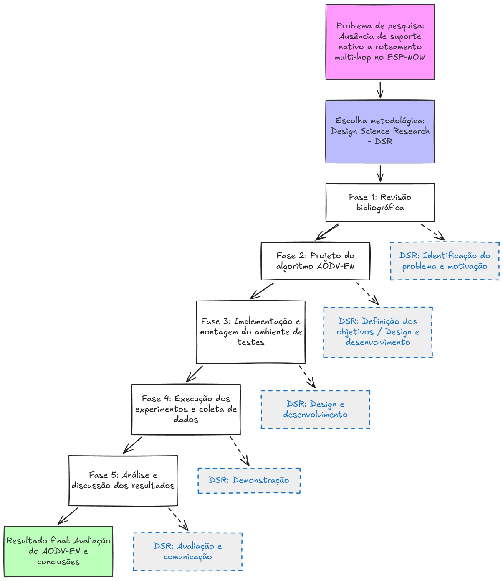
\includegraphics[keepaspectratio,alt={Figura 1 -- Fluxo metodológico da pesquisa}]{figuras/image1.png}}
\caption{Figura 1 -- Fluxo metodológico da pesquisa}
\end{figure}

\subsection{Fase 1: Revisão
Bibliográfica}\label{fase-1-revisuxe3o-bibliogruxe1fica}

A primeira fase corresponde à etapa de Identificação do Problema e
Motivação da DSR. Nesta fase, foi realizado o levantamento bibliográfico
para fundamentar teoricamente o trabalho e identificar com precisão as
lacunas existentes na literatura. O levantamento bibliográfico
concentrou-se em três eixos temáticos: (i) o protocolo AODV e suas
variantes, tendo como referência primária a RFC 3561; (ii) o protocolo
ESP-NOW, suas características técnicas e limitações; e (iii) soluções
existentes para redes mesh em plataformas embarcadas de baixo custo. As
fontes consultadas incluíram bases de dados científicas (IEEE Xplore,
ACM Digital Library, ScienceDirect), documentação técnica oficial
(Espressif Systems, IETF RFCs) e repositórios de projetos open-source
(GitHub). Os critérios de seleção priorizaram publicações recentes
(2021-2025) que abordassem especificamente ESP-NOW ou roteamento em
redes de sensores de baixo custo.

\subsection{Fase 2: Projeto do Algoritmo
AODV-EN}\label{fase-2-projeto-do-algoritmo-aodv-en}

A segunda fase corresponde às etapas de Definição dos Objetivos da
Solução e início do Design e Desenvolvimento. Nesta fase, são
especificados os requisitos funcionais e não-funcionais do artefato,
definida sua arquitetura e projetadas as adaptações necessárias do
protocolo AODV original para operação sobre ESP-NOW. O projeto do
AODV-EN parte dos princípios do protocolo AODV, especialmente quanto à
descoberta de rotas sob demanda, ao uso de mensagens de controle, à
manutenção de tabelas de roteamento e ao tratamento de falhas de enlace.
A partir desses princípios, foram definidas adaptações necessárias para
sua operação sobre ESP-NOW. As principais decisões de projeto incluem:
a) \textbf{Gerenciamento de peers}: política LRU (Least Recently Used)
para gerenciamento dinâmico da tabela de peers, permitindo comunicação
com mais de 20 nós ao longo do tempo dentro do limite simultâneo imposto
pelo ESP-NOW; b) \textbf{Disseminação de mensagens RREQ}:
\emph{flooding} controlado sobre \emph{broadcast} de enlace do ESP-NOW
(FF:FF:FF:FF:FF:FF), com supressão de duplicatas por cache de
identificadores e limite de propagação por TTL, preservando a semântica
de difusão do AODV original; c) \textbf{Métrica de roteamento}: métrica
híbrida combinando contagem de saltos (hop count) e qualidade de enlace
(RSSI), permitindo seleção de rotas que otimizem simultaneamente
distância lógica e confiabilidade esperada; d) \textbf{Estruturas de
dados}: tabela de roteamento, tabela de peers com timestamps, buffer de
RREQ IDs para detecção de duplicatas, e lista de precursores para
notificação de falhas.

\subsection{Fase 3: Implementação e Montagem do Ambiente de
Testes}\label{fase-3-implementauxe7uxe3o-e-montagem-do-ambiente-de-testes}

A terceira fase dá continuidade à etapa de Design e Desenvolvimento,
materializando o projeto em código funcional e preparando o ambiente
para os experimentos. A implementação será realizada em linguagem C
utilizando o framework ESP-IDF (Espressif IoT Development Framework). O
código será organizado em módulos: gerenciamento de peers, descoberta de
rotas, manutenção de rotas, encaminhamento de pacotes e interface de
coleta de métricas. Paralelamente, será implementado o algoritmo
Flooding para fins de comparação. O ambiente de testes (testbed) será
composto por 10 módulos ESP32 DevKit V1, alimentados por fontes USB 5V.
A disposição física dos nós seguirá as topologias definidas na Seção
4.4. Cada nó executará o mesmo firmware, sendo configurado com
identificador único através de variáveis de compilação.

\subsection{Fase 4: Execução dos Experimentos e Coleta de
Dados}\label{fase-4-execuuxe7uxe3o-dos-experimentos-e-coleta-de-dados}

A quarta fase corresponde à etapa de Demonstração da DSR, onde o
artefato é exercitado em cenários representativos para demonstrar sua
eficácia na resolução do problema. Os experimentos seguirão o
planejamento detalhado na Seção 4.4. Para cada cenário experimental,
serão realizadas múltiplas execuções (mínimo de 30 repetições) para
garantir significância estatística. As métricas serão coletadas
automaticamente pelo firmware e transmitidas para um nó coordenador, que
as registra em arquivos de log para posterior análise.

\subsection{Fase 5: Análise e Discussão dos
Resultados}\label{fase-5-anuxe1lise-e-discussuxe3o-dos-resultados}

A quinta fase corresponde às etapas de Avaliação e Comunicação da DSR.
Os dados coletados serão submetidos a análise estatística utilizando
técnicas descritivas (média, desvio padrão, intervalos de confiança) e
inferenciais (testes de hipóteses) quando apropriado. A avaliação
comparará os resultados do AODV-EN com: (i) o algoritmo Flooding
implementado localmente; e (ii) resultados reportados na literatura para
soluções similares, como o BRAM-NOW de Cujilema et al.~(2023). A
comunicação dos resultados será realizada através deste TCC e,
potencialmente, através de publicação em evento científico.

\section{Planejamento Experimental}\label{planejamento-experimental}

O planejamento experimental foi definido com o objetivo de avaliar o
comportamento do algoritmo AODV-EN em diferentes condições de operação
de uma rede mesh baseada em ESP-NOW. Considerando que a proposta envolve
roteamento multi-hop, seleção de rotas, manutenção da comunicação e
recuperação diante de falhas, os experimentos foram organizados em
cenários capazes de representar situações progressivamente mais
complexas de comunicação multi-hop. A avaliação será realizada por meio
da comparação entre o AODV-EN e um algoritmo de referência baseado em
Flooding, permitindo observar diferenças quanto à confiabilidade da
entrega, latência fim-a-fim, carga de controle e consumo energético
estimado.

\subsection{Cenários experimentais}\label{cenuxe1rios-experimentais}

Os experimentos serão conduzidos em quatro cenários distintos,
projetados para avaliar aspectos complementares do desempenho do
algoritmo proposto. O cenário C1 avalia o comportamento multi-hop básico
em uma topologia linear; o cenário C2 verifica o encaminhamento em uma
estrutura hierárquica; o cenário C3 analisa a seleção de rotas em uma
malha parcial com caminhos alternativos; e o cenário C4 observa a
capacidade de detecção de falhas e recuperação da comunicação.

\textbf{Quadro 9 -- Configuração dos cenários experimentais}

{\def\LTcaptype{none} % do not increment counter
\begin{longtable}[]{@{}
  >{\raggedright\arraybackslash}p{(\linewidth - 6\tabcolsep) * \real{0.2500}}
  >{\raggedright\arraybackslash}p{(\linewidth - 6\tabcolsep) * \real{0.2500}}
  >{\raggedright\arraybackslash}p{(\linewidth - 6\tabcolsep) * \real{0.2500}}
  >{\raggedright\arraybackslash}p{(\linewidth - 6\tabcolsep) * \real{0.2500}}@{}}
\toprule\noalign{}
\begin{minipage}[b]{\linewidth}\raggedright
Cenário
\end{minipage} & \begin{minipage}[b]{\linewidth}\raggedright
Topologia
\end{minipage} & \begin{minipage}[b]{\linewidth}\raggedright
Configuração
\end{minipage} & \begin{minipage}[b]{\linewidth}\raggedright
Objetivo
\end{minipage} \\
\midrule\noalign{}
\endhead
\bottomrule\noalign{}
\endlastfoot
C1: Linear & Cadeia & • 5 nós em linha (N1→N2→N3→N4→N5) • Distância
entre nós: 10m • Comunicação: N1↔N5 • 4 saltos obrigatórios & Avaliar
comportamento multi-hop básico e latência acumulada por salto \\
C2: Árvore & Hierárquica & • 7 nós em estrutura de árvore • 1 raiz, 2
nós nível 1, 4 folhas • Comunicação: folhas↔raiz • Máximo 2 saltos &
Avaliar encaminhamento hierárquico e agregação de tráfego \\
C3: Mesh Parcial & Redundante & • 6 nós com múltiplos caminhos • Cada nó
alcança 2-3 vizinhos • Comunicação: extremidades • Rotas alternativas
disponíveis & Avaliar seleção de rotas e capacidade de utilizar caminhos
alternativos \\
C4: Falha & Linear com interrupção & • Cenário C1 com falha induzida •
Nó N3 desligado após 60s • Observação da recuperação & Avaliar detecção
de falha e capacidade de auto-recuperação (self-healing) \\
\end{longtable}
}

Fonte: Elaborado pelos autores.

\subsection{Parâmetros dos
experimentos}\label{paruxe2metros-dos-experimentos}

Os parâmetros experimentais foram definidos com o objetivo de manter
condições equivalentes de comparação entre o AODV-EN e o algoritmo de
referência. Assim, variáveis como número de nós, tamanho do payload,
taxa de envio, duração das execuções e número de repetições foram
padronizadas para ambos os algoritmos, variando apenas os parâmetros
específicos de cada abordagem. No caso do AODV-EN, são considerados
parâmetros próprios do protocolo, como o intervalo de mensagens HELLO e
o tempo de validade das rotas ativas. Para o Flooding, define-se o valor
máximo de TTL, utilizado para limitar a propagação dos pacotes e evitar
retransmissões indefinidas.

\textbf{Quadro 10 -- Parâmetros dos experimentos}

{\def\LTcaptype{none} % do not increment counter
\begin{longtable}[]{@{}
  >{\centering\arraybackslash}p{(\linewidth - 4\tabcolsep) * \real{0.3333}}
  >{\centering\arraybackslash}p{(\linewidth - 4\tabcolsep) * \real{0.3333}}
  >{\centering\arraybackslash}p{(\linewidth - 4\tabcolsep) * \real{0.3333}}@{}}
\toprule\noalign{}
\begin{minipage}[b]{\linewidth}\centering
Parâmetro
\end{minipage} & \begin{minipage}[b]{\linewidth}\centering
AODV-EN
\end{minipage} & \begin{minipage}[b]{\linewidth}\centering
Flooding
\end{minipage} \\
\midrule\noalign{}
\endhead
\bottomrule\noalign{}
\endlastfoot
Número de nós & 5-10 (conforme cenário) & 5-10 (conforme cenário) \\
Tamanho do payload & 32 bytes & 32 bytes \\
Taxa de envio (steady state) & 1 pacote/segundo & 1 pacote/segundo \\
Duração de cada execução & 300 segundos (5 min) & 300 segundos (5
min) \\
Repetições por cenário & 30 & 30 \\
HELLO\_INTERVAL & 2.000 ms & N/A \\
ACTIVE\_ROUTE\_TIMEOUT & 10.000 ms & N/A \\
TTL máximo (Flooding) & N/A & 5 saltos \\
\end{longtable}
}

\section{}\label{section}

\section{}\label{section-1}

\section{}\label{section-2}

\section{}\label{section-3}

\section{}\label{section-4}

\section{}\label{section-5}

Fonte: Elaborado pelos autores.

\section{Métricas de Avaliação}\label{muxe9tricas-de-avaliauxe7uxe3o}

A avaliação do desempenho do algoritmo AODV-EN será realizada por meio
de quatro métricas complementares: Packet Delivery Ratio (PDR), latência
fim-a-fim, Normalized Routing Load (NRL) e consumo energético estimado.
Essas métricas foram selecionadas por sua recorrência na literatura de
redes ad-hoc e por sua adequação ao contexto de redes de sensores sem
fio com recursos limitados. O PDR permite avaliar a confiabilidade da
comunicação; a latência fim-a-fim indica o desempenho temporal da
entrega dos pacotes; o NRL mede o overhead de controle introduzido pelo
protocolo; e o consumo energético estimado permite analisar o impacto
das transmissões sobre a autonomia dos dispositivos.

\textbf{Quadro 11 -- Métricas de avaliação de desempenho}

{\def\LTcaptype{none} % do not increment counter
\begin{longtable}[]{@{}
  >{\raggedright\arraybackslash}p{(\linewidth - 4\tabcolsep) * \real{0.3333}}
  >{\raggedright\arraybackslash}p{(\linewidth - 4\tabcolsep) * \real{0.3333}}
  >{\raggedright\arraybackslash}p{(\linewidth - 4\tabcolsep) * \real{0.3333}}@{}}
\toprule\noalign{}
\begin{minipage}[b]{\linewidth}\raggedright
Métrica
\end{minipage} & \begin{minipage}[b]{\linewidth}\raggedright
Definição
\end{minipage} & \begin{minipage}[b]{\linewidth}\raggedright
Fórmula
\end{minipage} \\
\midrule\noalign{}
\endhead
\bottomrule\noalign{}
\endlastfoot
PDR (Packet Delivery Ratio) & Razão entre pacotes de dados recebidos no
destino e pacotes enviados pela origem. Indica a confiabilidade da
comunicação. & PDR = (Pacotes recebidos / Pacotes enviados) × 100\% \\
Latência Fim-a-Fim & Tempo decorrido entre o envio de um pacote pela
origem e sua recepção no destino. Inclui tempo de processamento,
enfileiramento e transmissão em cada salto. & L = t\_recepção -
t\_envio \\
NRL (Normalized Routing Load) & Razão entre o número de pacotes de
controle transmitidos e o número de pacotes de dados entregues. Indica a
eficiência do protocolo em termos de overhead. & NRL = Pacotes de
controle / Pacotes de dados entregues \\
Consumo Energético Estimado & Estimativa do consumo de energia baseada
no número de transmissões e no perfil de consumo do ESP32. Permite
projetar autonomia com bateria. & E = Σ(N\_tx × E\_tx + N\_rx × E\_rx +
t\_idle × P\_idle) \\
\end{longtable}
}

Fonte: Elaborado pelos autores.

Para cada métrica, serão calculados: média aritmética, desvio padrão e
intervalo de confiança de 95\%. Os resultados serão apresentados em
tabelas e gráficos comparativos entre AODV-EN e Flooding.

\section{Algoritmo de Referência para Comparação:
Flooding}\label{algoritmo-de-referuxeancia-para-comparauxe7uxe3o-flooding}

Para estabelecer uma base de comparação experimental, será implementado
um algoritmo de referência baseado em Flooding sobre ESP-NOW. O Flooding
é a abordagem mais básica para disseminação de mensagens em redes sem
infraestrutura, consistindo na retransmissão de cada pacote recebido
para todos os vizinhos, exceto aquele de quem o pacote foi recebido.

\subsection{Especificação do algoritmo
Flooding}\label{especificauxe7uxe3o-do-algoritmo-flooding}

O algoritmo de referência baseado em Flooding será implementado com as
seguintes características: a) \textbf{Estrutura do pacote}: cada pacote
contém identificador único (origem + número de sequência), endereço de
origem, endereço de destino, TTL (Time-To-Live) e payload de dados; b)
\textbf{Detecção de duplicatas}: cada nó mantém um buffer circular com
os últimos N identificadores de pacotes recebidos (N=100). Pacotes com
identificadores já presentes no buffer são descartados; c)
\textbf{Controle de TTL}: o TTL é decrementado a cada salto. Pacotes com
TTL=0 não são retransmitidos, limitando o alcance do flooding e
prevenindo loops infinitos; d) \textbf{Retransmissão}: ao receber um
pacote não-duplicado com TTL\textgreater0 e destino diferente do próprio
nó, o pacote é retransmitido em um único \emph{broadcast} de enlace
ESP-NOW (FF:FF:FF:FF:FF:FF), conforme a definição clássica de
\emph{flooding} --- uma retransmissão por nó, suprimida por duplicatas e
limitada por TTL; e) \textbf{Entrega ao destino}: quando o pacote
alcança o nó de destino, o payload é entregue à aplicação e a recepção é
registrada para cálculo das métricas.

\subsection{Justificativa da escolha do Flooding como algoritmo de
referência}\label{justificativa-da-escolha-do-flooding-como-algoritmo-de-referuxeancia}

A escolha do Flooding como algoritmo de comparação justifica-se por: a)
\textbf{Simplicidade}: é o algoritmo mais simples possível para
comunicação multi-hop, servindo como limite inferior de complexidade de
implementação; b) \textbf{Garantia de entrega}: em redes conectadas, o
Flooding garante que o pacote alcançará o destino (se existir caminho),
servindo como referência de PDR máximo alcançável; c) \textbf{Overhead
elevado}: o Flooding representa o extremo oposto em termos de
eficiência, permitindo quantificar os ganhos obtidos pelo roteamento
inteligente do AODV-EN; d) \textbf{Ausência de estado}: não requer
tabelas de roteamento ou manutenção de rotas, isolando o impacto desses
mecanismos no AODV-EN. A comparação entre o AODV-EN e o Flooding
permitirá avaliar a relação entre complexidade de implementação e
eficiência de comunicação. Embora o AODV-EN apresente maior complexidade
por envolver descoberta e manutenção de rotas, espera-se que ele
proporcione menor carga de controle, menor consumo energético estimado e
desempenho comparável em termos de taxa de entrega de pacotes.

\section{Coleta e Análise dos
Dados}\label{coleta-e-anuxe1lise-dos-dados}

Os dados experimentais serão coletados a partir dos registros gerados
durante a execução dos cenários de teste. Esses registros incluirão
informações sobre pacotes enviados, pacotes recebidos, mensagens de
controle, eventos de retransmissão, falhas de comunicação, atualizações
de rota e tempos de envio e recepção.
\begin{figure}[H]
\centering
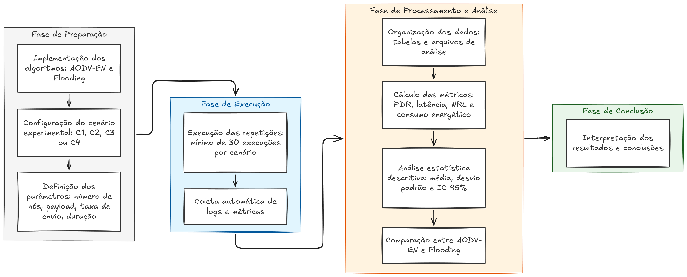
\includegraphics[width=0.85\textwidth,keepaspectratio]{figuras/image2.png}
\caption{Figura 2 -- Fluxo de execução dos experimentos e análise dos dados}
\end{figure}
A Figura 2 sintetiza o fluxo de execução dos experimentos e de
tratamento dos dados, desde a configuração do ambiente experimental até
a comparação dos resultados obtidos para o AODV-EN e o algoritmo de
referência baseado em Flooding. Para garantir a rastreabilidade dos
experimentos, cada execução deverá ser identificada pelo cenário
avaliado, algoritmo utilizado, número da repetição, configuração dos nós
e arquivos de log correspondentes. Essa organização permitirá relacionar
os resultados obtidos às condições específicas de cada execução
experimental. Após a coleta, os dados serão organizados em tabelas e
submetidos à análise estatística descritiva, considerando média, desvio
padrão e intervalo de confiança de 95\% para cada métrica avaliada. A
análise será realizada por cenário e por algoritmo, possibilitando a
comparação direta entre os resultados do AODV-EN e do algoritmo de
referência baseado em Flooding. Execuções com falhas de instrumentação,
perda de registros, reinicialização inesperada dos dispositivos ou
divergência de configuração serão desconsideradas e repetidas, a fim de
preservar a consistência dos dados analisados. A partir dos resultados
consolidados, será avaliado se o AODV-EN, apresenta ganhos em eficiência
de comunicação, mantendo desempenho compatível em termos de
confiabilidade e latência.

% -----------------------------------------------------------------------------
% Conteudo AODV-EN. Template base: Prof. Wesley Pacheco Calixto (IFG).
% -----------------------------------------------------------------------------
\chapter{PROJETO E IMPLEMENTAÇÃO DO ALGORITMO
AODV-EN}\label{projeto-e-implementauxe7uxe3o-do-algoritmo-aodv-en}

Este capítulo apresenta o projeto e a implementação do algoritmo
AODV-EN, desenvolvido como uma adaptação do protocolo AODV para redes
mesh baseadas em ESP-NOW. A apresentação foi organizada de forma
progressiva, partindo da visão geral da arquitetura até os mecanismos
internos de descoberta de rotas, encaminhamento de dados, manutenção de
rotas e tratamento de falhas. Ao final, são discutidas as principais
adaptações realizadas em relação ao AODV original, considerando as
restrições específicas do ESP-NOW. \#\# Visão Geral da Arquitetura do
AODV-EN A arquitetura do AODV-EN foi concebida em camadas, de modo a
separar as responsabilidades entre aplicação, interface pública de
integração, núcleo do protocolo, adaptador de transporte e meio de
comunicação ESP-NOW. Essa separação reduz o acoplamento entre os
componentes, favorece a manutenção do código e permite a evolução
incremental do artefato sem comprometer o funcionamento global da
solução. A Figura 3 apresenta a organização geral da arquitetura
proposta, evidenciando o fluxo de interação entre as camadas
responsáveis pela aplicação, pela interface pública da pilha, pelo
núcleo do protocolo, pelo adaptador de transporte e pelo meio de
comunicação ESP-NOW.
\begin{figure}[H]
\centering
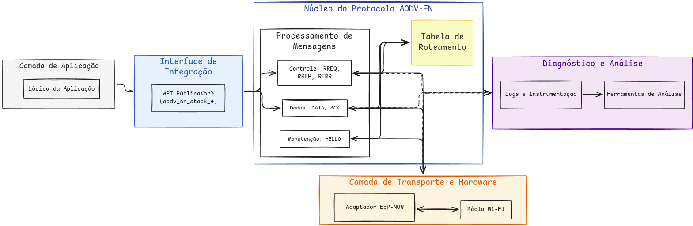
\includegraphics[width=0.85\textwidth,keepaspectratio]{figuras/image3.png}
\caption{Figura 3 -- Arquitetura geral do AODV-EN}
\end{figure}
A camada de aplicação é responsável por acionar o envio de dados e
registrar eventos de execução. A interface pública disponibiliza as
funções de inicialização, envio, recepção e atualização temporal da
pilha. O núcleo do protocolo concentra a lógica de roteamento, incluindo
descoberta de rotas, manutenção de tabelas, tratamento de falhas e
encaminhamento de pacotes. O adaptador ESP-NOW, por sua vez, encapsula
os detalhes de transmissão e recepção na camada de enlace.

\section{Estrutura Modular da
Implementação}\label{estrutura-modular-da-implementauxe7uxe3o}

A implementação do AODV-EN foi organizada em módulos funcionais com
interfaces explícitas, buscando separar a lógica central do protocolo
das estruturas auxiliares e dos detalhes específicos do transporte. Essa
organização contribui para a manutenção do código, facilita a validação
isolada de componentes e permite maior rastreabilidade entre as decisões
de projeto e sua materialização no firmware. A interface pública da
pilha é concentrada nos módulos aodv\_en.h e aodv\_en.c, responsáveis
por expor funções de inicialização, envio, recepção, atualização
temporal e consulta de estatísticas. O núcleo do protocolo é
implementado principalmente no módulo aodv\_en\_node.c, que coordena os
processos de descoberta de rotas, encaminhamento de dados, manutenção de
estados e tratamento de mensagens. Os demais módulos implementam
estruturas de apoio, como tabela de rotas, tabela de vizinhos, cache de
RREQ, gerenciamento de peers e manipulação de endereços MAC. A Figura 4
apresenta a organização modular da implementação, evidenciando a relação
entre a aplicação, a fachada pública da pilha, o núcleo do protocolo, os
módulos auxiliares e o adaptador ESP-NOW.
\begin{figure}[H]
\centering
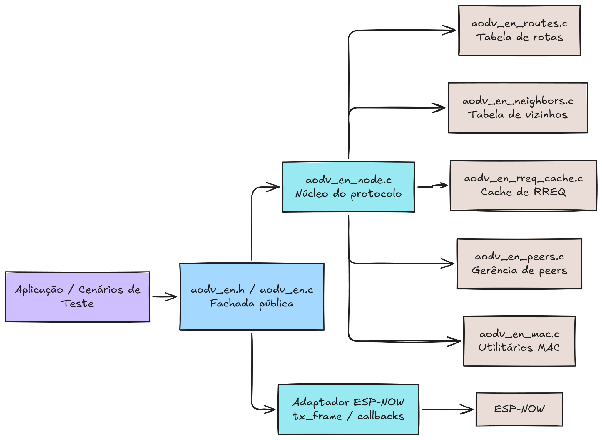
\includegraphics[width=0.85\textwidth,keepaspectratio]{figuras/image4.png}
\caption{Figura 4 -- Estrutura modular da implementação do AODV-EN}
\end{figure}

\section{Estruturas de Dados
Utilizadas}\label{estruturas-de-dados-utilizadas}

As estruturas de dados do AODV-EN foram projetadas considerando as
limitações de memória do ambiente embarcado e a necessidade de
atualização em tempo real das informações de roteamento. Essas
estruturas armazenam o estado local de cada nó e permitem a execução dos
mecanismos de descoberta, seleção, manutenção e invalidação de rotas. O
Quadro 12 apresenta uma síntese das principais estruturas utilizadas na
implementação do AODV-EN e sua função no funcionamento do protocolo.
\textbf{Quadro 12 -- Estruturas de dados utilizadas no AODV-EN}

{\def\LTcaptype{none} % do not increment counter
\begin{longtable}[]{@{}
  >{\raggedright\arraybackslash}p{(\linewidth - 4\tabcolsep) * \real{0.3333}}
  >{\raggedright\arraybackslash}p{(\linewidth - 4\tabcolsep) * \real{0.3333}}
  >{\raggedright\arraybackslash}p{(\linewidth - 4\tabcolsep) * \real{0.3333}}@{}}
\toprule\noalign{}
\begin{minipage}[b]{\linewidth}\raggedright
Estrutura
\end{minipage} & \begin{minipage}[b]{\linewidth}\raggedright
Função principal
\end{minipage} & \begin{minipage}[b]{\linewidth}\raggedright
Papel no protocolo
\end{minipage} \\
\midrule\noalign{}
\endhead
\bottomrule\noalign{}
\endlastfoot
Tabela de rotas & Armazenar destinos conhecidos, próximo salto, estado,
métrica e expiração & Permite seleção e encaminhamento de pacotes por
rotas válidas \\
Tabela de vizinhos & Registrar nós alcançáveis diretamente e informações
de RSSI & Subsidia o cálculo da métrica híbrida e a manutenção da
conectividade local \\
Cache de RREQ & Armazenar requisições de rota já processadas & Evita
duplicatas, retransmissões desnecessárias e ciclos de propagação \\
Gerenciamento de peers & Controlar pares registrados no ESP-NOW &
Permite operar dentro das limitações de peers simultâneos do ESP-NOW \\
\end{longtable}
}

\textbf{Fonte: Elaborado pelos autores.}

\subsection{Tabela de Rotas}\label{tabela-de-rotas}

\begin{verbatim}
A tabela de rotas mantém, para cada destino conhecido, informações como próximo salto, número de saltos, número de sequência, estado da rota, métrica de custo e tempo de expiração. Essa estrutura é essencial para o encaminhamento de pacotes, pois permite identificar se existe uma rota válida para determinado destino e qual vizinho deve ser utilizado como próximo salto.
\end{verbatim}

A atualização das entradas considera critérios de frescor da informação,
qualidade da rota e validade temporal, preservando o princípio do AODV
de priorizar rotas mais recentes e evitar informações obsoletas. Além
disso, a implementação emprega critérios de substituição que consideram
número de sequência, métrica, contagem de saltos e tempo de expiração,
reduzindo trocas instáveis de rota e contribuindo para maior
estabilidade do protocolo.

\subsection{Tabela de Vizinhos}\label{tabela-de-vizinhos}

A tabela de vizinhos registra os nós alcançáveis diretamente por um
determinado nó da rede. Para cada vizinho, são armazenadas informações
como endereço MAC, estado do enlace, último RSSI observado, RSSI médio,
instante da última comunicação e eventos de falha de enlace.

Essa estrutura subsidia tanto o encaminhamento local quanto o cálculo da
métrica híbrida de roteamento. Ao considerar informações de RSSI, o
AODV-EN pode avaliar não apenas a quantidade de saltos até o destino,
mas também a qualidade dos enlaces utilizados no caminho, favorecendo
rotas potencialmente mais estáveis em ambientes sem fio sujeitos a
interferências e variações de sinal.

\subsection{Cache de RREQ}\label{cache-de-rreq}

O cache de RREQ armazena pares formados pelo endereço do nó originador e
pelo identificador da requisição de rota. Esse mecanismo permite
reconhecer requisições já processadas, evitando que uma mesma mensagem
RREQ seja tratada repetidamente por um nó.

A utilização desse cache é fundamental em processos de flooding
controlado, pois reduz retransmissões redundantes, limita a propagação
excessiva de mensagens de controle e contribui para prevenir ciclos
durante a descoberta de rotas. Dessa forma, o cache de RREQ atua como
mecanismo de controle de overhead e de estabilidade do processo de
descoberta.

\subsection{Gerenciamento de Peers}\label{gerenciamento-de-peers}

O gerenciamento de peers foi projetado para lidar com a limitação de
pares simultâneos imposta pelo ESP-NOW. Como o protocolo exige que
dispositivos sejam registrados como peers para comunicação unicast, essa
restrição pode limitar a escalabilidade da rede quando há múltiplos nós
participantes.

Para contornar essa limitação, o AODV-EN separa a vizinhança lógica
mantida pelo protocolo da tabela física de peers utilizada pelo ESP-NOW.
Quando necessário, aplica-se uma política LRU (Least Recently Used),
substituindo pares menos recentemente utilizados e permitindo que o
protocolo opere com um número de nós maior que o limite simultâneo de
peers registrados. Essa estratégia preserva a compatibilidade com o
ESP-NOW sem comprometer a dinâmica de descoberta e manutenção de rotas.

\section{Mensagens do Protocolo}\label{mensagens-do-protocolo}

O AODV-EN utiliza mensagens de controle e de dados para realizar a
descoberta, manutenção e utilização das rotas na rede. As mensagens de
controle são responsáveis por estabelecer caminhos, atualizar estados,
manter a conectividade local e tratar falhas de enlace. Já as mensagens
de dados transportam a carga útil da aplicação entre origem e destino,
utilizando as rotas previamente descobertas pelo protocolo. A definição
dessas mensagens foi baseada nos princípios do AODV, especialmente
quanto ao uso de requisições de rota, respostas de rota e mensagens de
erro. Entretanto, foram incorporadas adaptações necessárias ao contexto
do ESP-NOW, como o uso de endereçamento por MAC, limitação de tamanho de
payload, controle de TTL e suporte à confirmação em nível de aplicação.
O Quadro 13 apresenta uma síntese das mensagens utilizadas pelo AODV-EN
e suas respectivas funções no protocolo. \textbf{Quadro 13 -- Mensagens
utilizadas pelo AODV-EN}

{\def\LTcaptype{none} % do not increment counter
\begin{longtable}[]{@{}
  >{\raggedright\arraybackslash}p{(\linewidth - 6\tabcolsep) * \real{0.2500}}
  >{\raggedright\arraybackslash}p{(\linewidth - 6\tabcolsep) * \real{0.2500}}
  >{\raggedright\arraybackslash}p{(\linewidth - 6\tabcolsep) * \real{0.2500}}
  >{\raggedright\arraybackslash}p{(\linewidth - 6\tabcolsep) * \real{0.2500}}@{}}
\toprule\noalign{}
\begin{minipage}[b]{\linewidth}\raggedright
Mensagem
\end{minipage} & \begin{minipage}[b]{\linewidth}\raggedright
Tipo
\end{minipage} & \begin{minipage}[b]{\linewidth}\raggedright
Função principal
\end{minipage} & \begin{minipage}[b]{\linewidth}\raggedright
Uso no protocolo
\end{minipage} \\
\midrule\noalign{}
\endhead
\bottomrule\noalign{}
\endlastfoot
RREQ & Controle & Requisitar descoberta de rota & Emitida quando um nó
precisa alcançar um destino para o qual não possui rota válida \\
RREP & Controle & Responder a uma requisição de rota & Retorna pelo
caminho reverso para estabelecer ou atualizar a rota até o destino \\
RERR & Controle & Notificar erro ou quebra de rota & Informa falhas de
enlace e permite invalidar rotas afetadas \\
HELLO & Controle & Manter vizinhança local & Atualiza a conectividade
entre nós diretamente alcançáveis \\
DATA & Dados & Transportar a carga útil da aplicação & Encaminhada salto
a salto conforme a tabela de rotas \\
ACK & Controle/aplicação & Confirmar recebimento de dados & Apoia a
verificação de entrega e o cálculo de métricas de confiabilidade \\
\end{longtable}
}

\textbf{Fonte: Elaborado pelos autores.}

As mensagens RREQ, RREP e RERR compõem o núcleo do mecanismo de
roteamento reativo do AODV-EN. A mensagem RREQ é utilizada quando a
origem necessita descobrir uma rota para determinado destino. Ao ser
propagada pela rede, ela permite que os nós intermediários estabeleçam
rotas reversas para a origem. A mensagem RREP, por sua vez, retorna pelo
caminho reverso e permite a formação da rota direta até o destino. Já a
mensagem RERR é utilizada quando ocorre falha de enlace ou invalidação
de rota, permitindo que os nós afetados atualizem suas tabelas e iniciem
nova descoberta, se necessário.

A mensagem HELLO é utilizada para manutenção da vizinhança local,
permitindo identificar nós diretamente alcançáveis e atualizar
informações associadas aos enlaces. Essas informações são importantes
para a manutenção das rotas e para o cálculo da métrica híbrida baseada
em número de saltos e qualidade do sinal.

As mensagens DATA e ACK estão associadas à comunicação da aplicação. A
mensagem DATA transporta a carga útil entre origem e destino, utilizando
as rotas válidas mantidas pelo protocolo. Quando necessário, a mensagem
ACK confirma o recebimento dos dados em nível de aplicação, contribuindo
para a avaliação da confiabilidade da entrega e para o controle de
retransmissões.

\section{Funcionamento do Algoritmo}\label{funcionamento-do-algoritmo}

O funcionamento do AODV-EN pode ser compreendido a partir de quatro
processos principais: descoberta de rotas, encaminhamento de dados,
manutenção de rotas e tratamento de falhas. Esses processos operam de
forma integrada para permitir a comunicação multi-hop em redes baseadas
em ESP-NOW, preservando a característica reativa do protocolo AODV
original. De modo geral, quando um nó precisa enviar dados para um
destino e não possui rota válida, o protocolo inicia um processo de
descoberta de rota. Após a definição do caminho, os pacotes de dados são
encaminhados de salto a salto até o destino. Durante a operação da rede,
mecanismos de manutenção verificam a validade das rotas e a
conectividade entre vizinhos. Caso ocorra falha de enlace, as rotas
afetadas são invalidadas e uma nova descoberta pode ser iniciada. \#\#\#
Descoberta de Rotas A descoberta de rotas é iniciada quando um nó de
origem precisa enviar dados para um destino e não possui uma rota válida
em sua tabela de roteamento. Nessa situação, o nó originador emite uma
mensagem RREQ contendo informações como endereço de origem, endereço de
destino, identificador da requisição, número de sequência e limite de
propagação. Ao receber uma mensagem RREQ, cada nó intermediário verifica
se a requisição já foi processada anteriormente. Caso seja uma
requisição duplicada, ela é descartada. Caso contrário, o nó registra ou
atualiza uma rota reversa para a origem, incrementa o contador de saltos
e retransmite a requisição conforme a política de disseminação
configurada. Quando a mensagem RREQ alcança o destino, ou um nó que
possua rota válida para ele, é gerada uma mensagem RREP. Essa resposta
retorna em unicast pelo caminho reverso previamente estabelecido,
permitindo que os nós intermediários atualizem suas rotas diretas até o
destino. Ao receber o RREP, a origem passa a possuir uma rota válida e
pode iniciar o envio dos dados pendentes. A Figura 5 apresenta o fluxo
de descoberta de rotas no AODV-EN, destacando a propagação da mensagem
RREQ e o retorno da mensagem RREP pelo caminho reverso.
\begin{figure}[H]
\centering
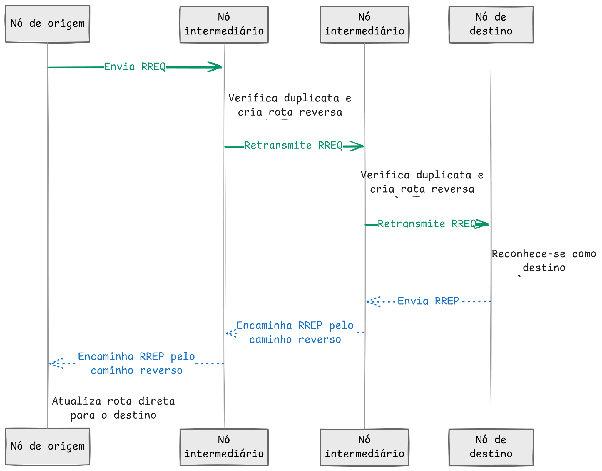
\includegraphics[width=0.85\textwidth,keepaspectratio]{figuras/image5.png}
\caption{Figura 5 -- Fluxo de descoberta de rotas no AODV-EN}
\end{figure}
\#\#\# Encaminhamento de Dados Após a descoberta de uma rota válida, o
encaminhamento dos dados ocorre de forma salto a salto. O nó de origem
consulta sua tabela de rotas para identificar o próximo salto em direção
ao destino e transmite a mensagem DATA ao vizinho correspondente. Cada
nó intermediário repete o mesmo procedimento, consultando sua própria
tabela de rotas até que o pacote alcance o destino final. Caso a origem
não possua rota válida no momento da tentativa de envio, o pacote é
armazenado temporariamente em uma fila de dados pendentes. Em seguida, o
protocolo inicia o processo de descoberta de rota por meio do envio de
uma mensagem RREQ. Quando a rota é estabelecida, os dados pendentes são
transmitidos conforme o caminho descoberto. Esse mecanismo permite que a
aplicação solicite o envio de dados mesmo quando a rota ainda não está
disponível, preservando a característica reativa do AODV-EN e evitando o
descarte imediato de pacotes em situações de descoberta inicial.

\subsection{Manutenção de Rotas}\label{manutenuxe7uxe3o-de-rotas}

A manutenção de rotas tem como objetivo preservar a validade das
informações de roteamento durante a operação da rede. Para isso, o
AODV-EN utiliza mecanismos de controle baseados em mensagens periódicas,
temporizadores de expiração e atualização do estado dos vizinhos. As
mensagens HELLO são utilizadas para manter a conectividade local entre
nós diretamente alcançáveis. A partir dessas mensagens, cada nó atualiza
sua tabela de vizinhos, registrando informações como instante da última
comunicação, estado do enlace e intensidade do sinal recebido. Essas
informações contribuem para identificar vizinhos ativos e subsidiar o
cálculo da métrica híbrida de roteamento. Além da manutenção da
vizinhança, cada rota possui um tempo de validade associado. Rotas que
permanecem sem uso ou ultrapassam seu tempo de expiração deixam de ser
consideradas válidas para encaminhamento. Esse mecanismo reduz o uso de
informações obsoletas e contribui para evitar encaminhamentos por
caminhos indisponíveis. A manutenção de rotas também está relacionada ao
controle de estabilidade. Ao atualizar uma rota existente, o protocolo
considera critérios como número de sequência, métrica, contagem de
saltos e tempo de expiração, evitando substituições frequentes quando a
nova rota não apresenta melhoria significativa. \#\#\# Tratamento de
Falhas O tratamento de falhas é acionado quando o protocolo identifica
indisponibilidade de um enlace ou impossibilidade de encaminhar dados
por uma rota previamente considerada válida. Essa detecção pode ocorrer
por ausência de resposta, falha de transmissão, expiração de vizinhança
ou perda de conectividade com o próximo salto. Ao detectar uma falha, o
nó invalida as rotas que dependem do enlace afetado e gera uma mensagem
RERR para notificar os nós impactados. Essa mensagem permite que os
demais nós atualizem suas tabelas de roteamento, evitando o uso de
caminhos inválidos. Quando ainda existem dados pendentes para o destino
afetado, o protocolo pode iniciar uma nova descoberta de rota por meio
de RREQ. Esse mecanismo permite que o AODV-EN reaja dinamicamente a
alterações na topologia da rede, buscando restabelecer a comunicação por
rotas alternativas quando disponíveis. Dessa forma, o tratamento de
falhas contribui para a capacidade de auto-recuperação da rede mesh. A
Figura 6 apresenta o fluxo de tratamento de falhas e reconvergência do
AODV-EN, desde a detecção da falha até a tentativa de restabelecimento
da comunicação.
\begin{figure}[H]
\centering
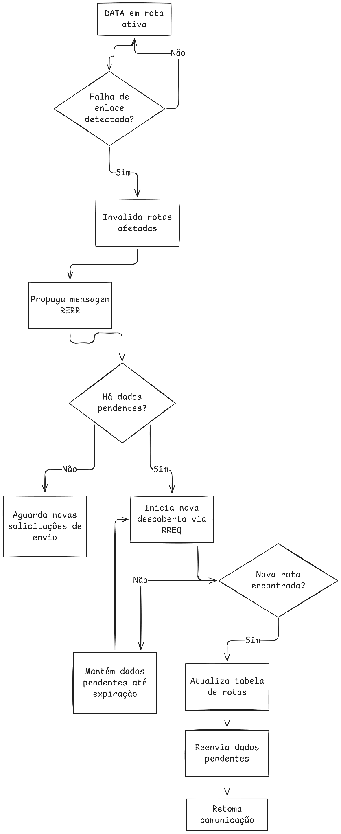
\includegraphics[width=0.85\textwidth,keepaspectratio]{figuras/image6.png}
\caption{Figura 6 -- Fluxo de tratamento de falhas e reconvergência no AODV-EN}
\end{figure}
\#\# Adaptações do AODV para ESP-NOW A adaptação do AODV para operação
sobre ESP-NOW exigiu modificações relacionadas ao endereçamento, à
disseminação de mensagens, ao gerenciamento de peers e à métrica de
seleção de rotas. Essas adaptações foram necessárias porque o ESP-NOW
opera na camada de enlace, utiliza endereçamento baseado em MAC, possui
limitação no número de peers registrados simultaneamente e não oferece,
de forma nativa, mecanismos completos para roteamento multi-hop. Dessa
forma, o AODV-EN preserva os princípios fundamentais do AODV, como
descoberta de rotas sob demanda, uso de mensagens de controle,
manutenção de tabelas de roteamento e tratamento de falhas, mas
incorpora mecanismos específicos para viabilizar sua execução em
dispositivos ESP32 utilizando ESP-NOW. O Quadro 14 sintetiza as
principais adaptações realizadas no AODV-EN em relação ao AODV original.
\textbf{Quadro 14 -- Principais adaptações do AODV para o contexto do
ESP-NOW}

{\def\LTcaptype{none} % do not increment counter
\begin{longtable}[]{@{}
  >{\raggedright\arraybackslash}p{(\linewidth - 4\tabcolsep) * \real{0.3333}}
  >{\raggedright\arraybackslash}p{(\linewidth - 4\tabcolsep) * \real{0.3333}}
  >{\raggedright\arraybackslash}p{(\linewidth - 4\tabcolsep) * \real{0.3333}}@{}}
\toprule\noalign{}
\begin{minipage}[b]{\linewidth}\raggedright
Aspecto
\end{minipage} & \begin{minipage}[b]{\linewidth}\raggedright
AODV original
\end{minipage} & \begin{minipage}[b]{\linewidth}\raggedright
Adaptação no AODV-EN
\end{minipage} \\
\midrule\noalign{}
\endhead
\bottomrule\noalign{}
\endlastfoot
Endereçamento & Utiliza endereçamento IP & Utiliza endereços MAC dos
dispositivos ESP32 \\
Disseminação de RREQ & Baseada em broadcast IP & Flooding controlado
sobre broadcast de enlace (MAC) com cache de duplicatas e TTL \\
Gerenciamento de vizinhos & Associado à conectividade da rede ad-hoc &
Mantém tabela de vizinhos com estado, último contato e RSSI \\
Gerenciamento de peers & Não aplicável diretamente ao AODV original &
Usa cache de peers e política LRU para lidar com o limite do ESP-NOW \\
Métrica de rota & Baseada principalmente em número de saltos & Combina
hop count e penalidade associada ao RSSI \\
Tratamento de falhas & Usa mensagens RERR e invalidação de rotas &
Mantém RERR, invalidação de rotas e redescoberta adaptada ao ESP-NOW \\
\end{longtable}
}

\textbf{Fonte: Elaborado pelos autores.}

\subsection{Endereçamento por MAC}\label{endereuxe7amento-por-mac}

No AODV original, o endereçamento dos nós é normalmente associado à
camada de rede, utilizando endereços IP para identificar origem, destino
e próximos saltos. No AODV-EN, essa lógica foi adaptada para o uso de
endereços MAC, uma vez que o ESP-NOW opera diretamente sobre a camada de
enlace do padrão IEEE 802.11. Essa adaptação permite que cada
dispositivo ESP32 seja identificado pelo seu endereço MAC, utilizado
tanto nas mensagens de controle quanto nas mensagens de dados. Assim,
campos como origem, destino, próximo salto e remetente do enlace são
representados por endereços MAC, preservando a semântica de roteamento
do AODV, mas adequando-a ao modelo de comunicação do ESP-NOW. A
utilização de endereçamento por MAC também simplifica a integração com o
mecanismo de envio do ESP-NOW, uma vez que a transmissão unicast exige a
indicação direta do endereço MAC do peer de destino. \#\#\# Flooding
Controlado sobre Broadcast de Enlace Uma das principais decisões de
projeto na adaptação do AODV ao ESP-NOW está relacionada à disseminação
das mensagens RREQ. No AODV original, a descoberta de rotas é realizada
por meio da difusão da requisição de rota pela rede, utilizando
broadcast. O ESP-NOW permite enviar quadros ao endereço de broadcast de
enlace (FF:FF:FF:FF:FF:FF), ainda que sem confirmação de entrega. O
AODV-EN adota a estratégia de flooding controlado sobre esse broadcast
de enlace: cada nó retransmite uma única vez cada RREQ novo recebido,
suprimindo duplicatas por meio do cache de identificadores (originador,
RREQ ID) e limitando a propagação pelo TTL. Essa abordagem preserva
fielmente a semântica de difusão do AODV e mantém a contagem de
transmissões simétrica em relação ao algoritmo de referência. Em uma
etapa intermediária do desenvolvimento, avaliou-se uma alternativa de
flooding por unicast sequencial, na qual o nó percorreria a tabela de
vizinhos e enviaria o RREQ individualmente a cada um, aproveitando a
confirmação de enlace do unicast ESP-NOW. Essa alternativa foi
descartada por introduzir um viés metodológico: o unicast ESP-NOW
realiza retransmissões automáticas em nível de MAC (confirmação CTS-ACK)
inexistentes no broadcast, o que inflaria artificialmente a
confiabilidade medida, subcontaria as transmissões reais (uma
transmissão lógica corresponderia a N quadros no ar) e descaracterizaria
a comparação com o flooding canônico. Optou-se, assim, pela disseminação
por broadcast de enlace, com confirmação realizada fim-a-fim por
mensagens ACK em nível de aplicação. \#\#\# Gerenciamento Dinâmico de
Peers O ESP-NOW impõe restrições quanto ao número de peers que podem ser
registrados simultaneamente para comunicação. Essa limitação afeta
diretamente a construção de redes mesh, pois o número total de nós
participantes pode ser superior ao número de peers mantidos fisicamente
pelo dispositivo em determinado instante. Para lidar com essa restrição,
o AODV-EN separa a vizinhança lógica utilizada pelo protocolo da tabela
física de peers mantida pelo ESP-NOW. A tabela de vizinhos representa os
nós conhecidos ou alcançáveis no contexto do roteamento, enquanto o
cache de peers controla quais dispositivos estão efetivamente
registrados para transmissão no momento. Quando a capacidade da tabela
de peers é atingida, aplica-se uma política LRU (Least Recently Used),
substituindo o peer menos recentemente utilizado por um novo peer
necessário à comunicação. Essa estratégia permite que o protocolo opere
dinamicamente em redes com mais nós do que o limite simultâneo de peers,
preservando a compatibilidade com o ESP-NOW e reduzindo a necessidade de
configuração manual da rede. \#\#\# Métrica Híbrida com Hop Count e RSSI
O AODV original utiliza, de forma predominante, a contagem de saltos
como critério de seleção de rotas. Essa abordagem favorece caminhos mais
curtos, mas pode desconsiderar a qualidade dos enlaces sem fio. Em redes
baseadas em ESP-NOW, essa limitação é relevante, pois enlaces com menor
número de saltos podem apresentar baixa qualidade de sinal, maior
instabilidade ou maior probabilidade de perda de pacotes. Para
considerar esse aspecto, o AODV-EN utiliza uma métrica híbrida que
combina a distância lógica da rota, representada pelo número de saltos,
com uma penalidade associada à qualidade do sinal recebido. A formulação
geral da métrica pode ser expressa por:

\begin{figure}[H]
\centering
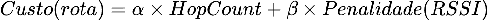
\includegraphics[width=0.85\textwidth,keepaspectratio]{figuras/image7.png}
\caption{Figura 7 - Fórmula do custo}
\end{figure}
Nessa formulação, α e β representam pesos configuráveis, HopCount
corresponde ao número de saltos até o destino e Penalidade(RSSI)
representa uma função de custo associada à qualidade média do enlace.
Quanto menor o número de saltos e melhor a qualidade do sinal, menor
tende a ser o custo da rota. Essa adaptação permite que a seleção de
rotas considere não apenas o caminho mais curto, mas também a robustez
dos enlaces envolvidos, contribuindo para maior estabilidade da
comunicação em ambientes sem fio sujeitos a interferências, obstáculos e
variações de sinal. \#\# Considerações sobre a Implementação A
implementação do AODV-EN buscou preservar os princípios fundamentais do
protocolo AODV, especialmente a descoberta de rotas sob demanda, a
manutenção de tabelas de roteamento, o uso de mensagens de controle e o
tratamento de falhas de enlace. Entretanto, devido às particularidades
do ESP-NOW, foram necessárias adaptações relacionadas ao endereçamento
por MAC, ao gerenciamento dinâmico de peers, à disseminação controlada
de requisições de rota e ao uso de métricas baseadas na qualidade do
enlace. Dessa forma, o algoritmo não corresponde a uma reprodução
literal do AODV original, mas a uma adaptação orientada às restrições de
comunicação, memória e operação do ESP32. A estrutura modular adotada
permite isolar responsabilidades, facilitar futuras extensões e fornecer
os dados necessários para a avaliação experimental.

% -----------------------------------------------------------------------------
% Conteudo AODV-EN. Template base: Prof. Wesley Pacheco Calixto (IFG).
% -----------------------------------------------------------------------------
\chapter{RESULTADOS E DISCUSSÃO}\label{cap:resultados}\label{resultados-e-discussuxe3o}

Este capítulo apresenta os resultados obtidos com a implementação e a
avaliação experimental do algoritmo AODV-EN, comparando-o ao algoritmo
de referência baseado em \emph{flooding}. Inicialmente, descreve-se o
ambiente de coleta e a validação funcional do protótipo. Em seguida,
apresentam-se os resultados de hardware para as quatro métricas
definidas na metodologia (PDR, latência, NRL e consumo energético
estimado), seguidos da análise de escalabilidade obtida por simulação.
Por fim, discutem-se a conformidade da implementação com a RFC 3561 e as
limitações do estudo.

\section{Ambiente das Coletas e Validação
Funcional}\label{ambiente-das-coletas-e-validauxe7uxe3o-funcional}

A avaliação experimental foi conduzida no cenário C1
(Seção~\ref{cenuxe1rios-experimentais}), com dez módulos ESP32-WROOM-32
dispostos em cadeia multi-hop ao longo de uma residência. A potência de
transmissão foi reduzida a 2~dBm para forçar a formação de múltiplos
saltos reais no espaço disponível, e a topologia foi verificada antes de
cada campanha por meio da matriz de RSSI da rede inteira, coletada por
telemetria em banda: cada nó reporta periodicamente seus vizinhos e o
respectivo RSSI ao coletor, que reconstrói a malha completa, inclusive os
nós que não são seus vizinhos diretos. Na topologia avaliada, o nó de
origem (também coletor, conectado à porta serial) alcançou o destino em
três a quatro saltos, com rota válida, percorrendo enlaces firmes
(−70 a −82~dBm) verificados na matriz.

Os parâmetros foram mantidos idênticos para os dois algoritmos:
\emph{payload} de 32 bytes, taxa de um pacote por segundo, uma origem
transmitindo a um destino fixo, janela de 60 segundos por repetição e
trinta repetições por algoritmo. Em vez de reinicializar fisicamente os
dez dispositivos espalhados a cada repetição, os contadores cumulativos
foram convertidos em medidas por janela no \emph{host}, tomando-se a
diferença entre o primeiro e o último reporte de cada nó na janela
(equivalente a um \emph{boot} lógico limpo por repetição, sem necessidade
de reprogramar nós sem cabo). A latência fim-a-fim foi medida na própria
origem, por RTT no mesmo relógio (\emph{esp\_timer}, em microssegundos),
eliminando a dependência de sincronização entre nós e a quantização
imposta por laços de aplicação.

Antes das coletas em hardware, o núcleo do protocolo foi validado por
meio de um conjunto de simulações determinísticas, executadas
diretamente a partir do código-fonte do componente, com rádio em memória
e relógio virtual. Essas simulações exercitam o ciclo completo de
descoberta (RREQ → RREP), encaminhamento de dados, confirmação fim-a-fim
(ACK) e propagação de erro de rota (RERR), além de cenários em grade de
até centenas de nós, garantindo que a lógica de roteamento se comporte
corretamente independentemente do hardware.

Para a coleta e a observação em tempo real dos experimentos, foi
desenvolvida uma ferramenta de monitoramento que lê as portas seriais
dos nós, interpreta os registros emitidos pelo \emph{firmware} e
apresenta, em um painel web, a topologia da malha, as tabelas de rotas,
os vizinhos com respectivo RSSI, os fluxos de dados e um console de
eventos. A ferramenta reconhece tanto o AODV-EN --- exibindo rotas
válidas, reversas e inválidas e as arestas de vizinhança --- quanto o
algoritmo de \emph{flooding} --- exibindo os fluxos de dados
origem-destino com o número de saltos percorridos. Um modo de reprodução
(\emph{replay}) permite reexecutar registros previamente capturados com
o ritmo temporal original, recurso utilizado para validar a interface
contra dados reais dos dois algoritmos.

\section{Resultados de Hardware}\label{resultados-de-hardware}

O desempenho dos dois algoritmos foi medido em trinta repetições por
algoritmo, sobre a mesma topologia física. Adotou-se como métrica
principal de confiabilidade a \emph{taxa de entrega} (PDR): pacotes
distintos efetivamente entregues à aplicação no nó de destino, divididos
pelos pacotes enviados pela origem --- definição usual na literatura de
redes \emph{ad hoc} e justa para os dois algoritmos, por contabilizar
apenas o que chegou ao destino, independentemente do caminho de volta. A
confirmação fim-a-fim por ACK é reportada como métrica secundária (taxa
de confirmação de ida e volta), por depender também da confiabilidade do
caminho reverso. Para o custo de canal, além da carga de roteamento
normalizada (NRL, mensagens de controle por dado entregue), reporta-se o
total de transmissões por pacote entregue, que captura de forma justa o
custo de ambos os algoritmos --- inclusive o das retransmissões por
inundação do \emph{flooding}, que a NRL clássica não contabiliza. O
conjunto bruto por repetição (incluindo os desvios padrão) está disponível
no repositório do projeto; a Tabela~\ref{tab:comparacao} consolida a média
e o intervalo de confiança de 95\% (IC95) de cada métrica.

\begin{table}[H]
\centering
\caption{Comparação AODV-EN vs.~Flooding em hardware --- cenário C1, 10 nós, multi-hop, 30 repetições (média $\pm$ intervalo de confiança de 95\%)}\label{tab:comparacao}
\begin{tabular}{@{}lcc@{}}
\toprule
Métrica & AODV-EN & Flooding (broadcast) \\
\midrule
PDR de entrega (\%) & 94,1 $\pm$ 1,4 & 12,7 $\pm$ 3,4 \\
PDR confirmação ida-volta (\%) & 91,7 $\pm$ 4,2 & 3,7 $\pm$ 0,8 \\
Latência one-way (ms) & 45,9 $\pm$ 3,5 & 31,6 $\pm$ 1,7 \\
NRL (controle de rota/entregue) & 18,0 $\pm$ 4,7 & 0,0 \\
Transmissões por entrega & 54,2 $\pm$ 10,1 & 102,9 $\pm$ 36,2 \\
Energia agregada (J, estimada) & 39,4 $\pm$ 0,6 & 28,4 $\pm$ 0,03 \\
\textbf{Energia por pacote entregue (J)} & \textbf{0,69 $\pm$ 0,02} & \textbf{5,66 $\pm$ 2,08} \\
\bottomrule
\end{tabular}

\vspace{2pt}
{\footnotesize Fonte: Elaborado pelos autores.}
\end{table}

A Figura~\ref{fig:hw-metrics} apresenta graficamente as quatro
dimensões comparadas (entrega, latência, transmissões por entrega e
energia estimada), com barras de erro correspondentes ao intervalo de
confiança de 95\% entre as trinta repetições.

\begin{figure}
\centering
\pandocbounded{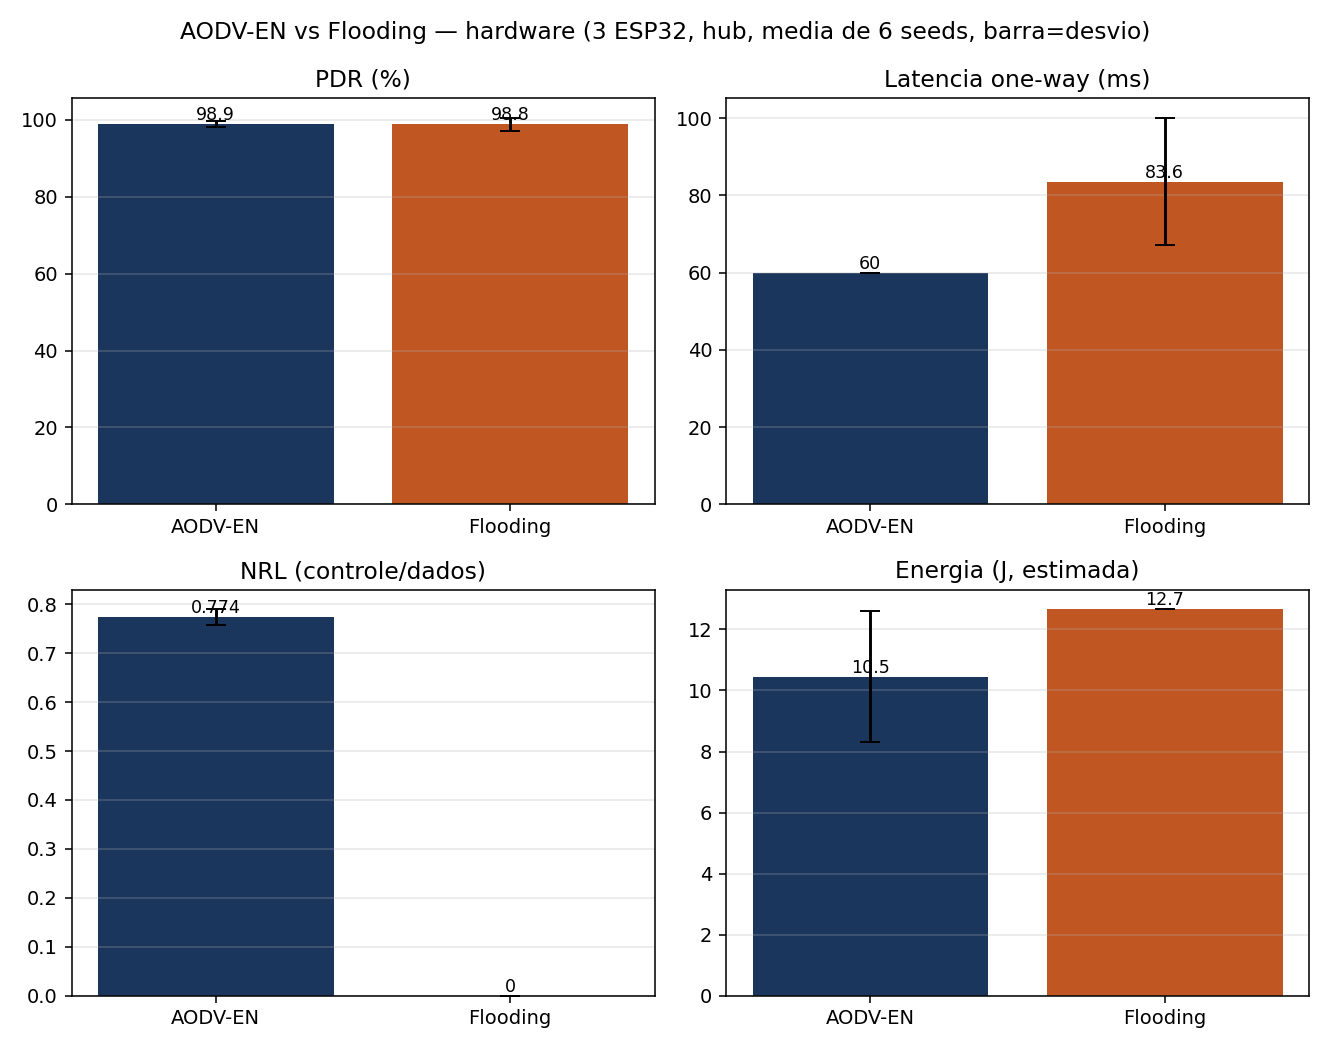
\includegraphics[keepaspectratio,alt={Métricas de hardware (PDR de entrega, latência, transmissões por entrega e energia): AODV-EN vs.~Flooding, média de 30 repetições com barra de IC95.}]{figuras/fig_hw_metrics.png}}
\caption{Métricas de hardware (PDR de entrega, latência, transmissões por
entrega e energia estimada): AODV-EN vs.~Flooding, cenário C1 multi-hop,
10 nós, média de 30 repetições com barra de IC95.}\label{fig:hw-metrics}
\end{figure}

\subsection{Significância estatística}\label{significuxe2ncia-estatuxedstica}

Para verificar se as diferenças observadas são estatisticamente
significativas, e não fruto da variabilidade amostral, aplicou-se a cada
métrica o teste $t$ de Welch (apropriado a variâncias desiguais) e, de
forma complementar, o teste não paramétrico de Mann--Whitney (que não
pressupõe normalidade), ambos bilaterais com nível de significância
$\alpha = 0{,}05$ e $n = 30$ repetições por algoritmo. A magnitude do
efeito foi quantificada pelo $d$ de Cohen. A Tabela~\ref{tab:stats}
resume os resultados.

\begin{table}[H]
\centering
\caption{Significância estatística das diferenças AODV-EN vs.~Flooding (cenário C1, $n=30$ por grupo)}\label{tab:stats}
\begin{tabular}{@{}lcccl@{}}
\toprule
Métrica & $t$ (Welch) & $p$ & $d$ de Cohen & Efeito \\
\midrule
PDR de entrega & 43,7 & $<0{,}001$ & 11,3 & altíssimo \\
Latência one-way & 7,2 & $<0{,}001$ & 1,85 & grande \\
NRL (controle/entregue) & 7,5 & $<0{,}001$ & 1,95 & grande \\
Transmissões por entrega & $-2{,}5$ & $0{,}011$ & $-0{,}71$ & médio \\
Energia (estimada) & 33,5 & $<0{,}001$ & 8,65 & altíssimo \\
\bottomrule
\end{tabular}

\vspace{2pt}
{\footnotesize Fonte: Elaborado pelos autores. Teste de Mann--Whitney concordante ($p<0{,}05$) em todas as métricas.}
\end{table}

Todas as diferenças são estatisticamente significativas ($p < 0{,}05$),
com os testes paramétrico e não paramétrico em concordância. Os tamanhos
de efeito da entrega ($d = 11{,}3$) e do consumo estimado ($d = 8{,}65$)
são muito superiores ao limiar convencional de efeito grande ($d > 0{,}8$),
indicando que a vantagem do AODV-EN na entrega multi-hop é estrutural, e
não marginal. A única diferença de efeito apenas médio é a de transmissões
por entrega ($d = -0{,}71$, $p = 0{,}011$), atenuada pela alta dispersão do
\emph{flooding} nessa métrica --- ainda assim significativa e desfavorável
ao \emph{flooding}.

\subsection{Distribuição entre repetições}\label{distribuiuxe7uxe3o-entre-repetiuxe7uxf5es}

A dispersão entre as repetições revela a \emph{estabilidade} de cada
algoritmo, informação que a média sozinha oculta. O AODV-EN entregou entre
85,2\% e 100\% dos pacotes (mediana 94,2\%; coeficiente de variação
$\mathrm{CV} = 4{,}2\%$), com apenas 4 das 30 repetições abaixo de 90\%. O
\emph{flooding}, em contraste, variou de 0\% a 36,2\% (mediana 10,7\%;
$\mathrm{CV} = 74{,}2\%$), com 20 das 30 repetições abaixo de 15\% e uma
repetição sem nenhuma entrega. A diferença de variabilidade --- CV de 4\%
contra 74\% --- mostra que o AODV-EN não apenas entrega mais, mas entrega de
forma previsível, ao passo que o \emph{flooding} colapsa de modo errático sob
as colisões da inundação a cada repetição.

\section{Discussão por Métrica}\label{discussuxe3o-por-muxe9trica}

\textbf{Confiabilidade (PDR).} No regime multi-hop (três a quatro
saltos), o AODV-EN entregou 94,1\% dos pacotes contra apenas 12,7\% do
\emph{flooding} --- diferença de grande magnitude e estatisticamente
inequívoca (intervalos de confiança disjuntos). O \emph{flooding} não
sobrevive ao multi-hop: sem rota nem retransmissão, cada pacote precisa
atravessar os saltos por difusão, e a probabilidade de sucesso decai
aproximadamente como o produto das probabilidades por enlace sob a
potência reduzida de 2~dBm. O descarte por TTL foi nulo, o que confirma
que a perda é de enlace --- colisões da tempestade de \emph{broadcast} e
ausência de confirmação --- e não de alcance fixo. O AODV-EN, ao
contrário, recupera perdas pela retransmissão fim-a-fim sobre a rota
estabelecida. A taxa de confirmação de ida e volta acentua o contraste
(91,7\% contra 3,7\%): além de entregar muito mais, o AODV-EN oferece
confirmação bidirecional confiável, propriedade ausente no
\emph{flooding}, cujo ACK também se difunde de volta e raramente completa
o trajeto de retorno. A Figura~\ref{fig:pdr-rep} evidencia, repetição a
repetição, a entrega alta e estável do AODV-EN frente à entrega baixa e
dispersa do \emph{flooding}.

\begin{figure}
\centering
\pandocbounded{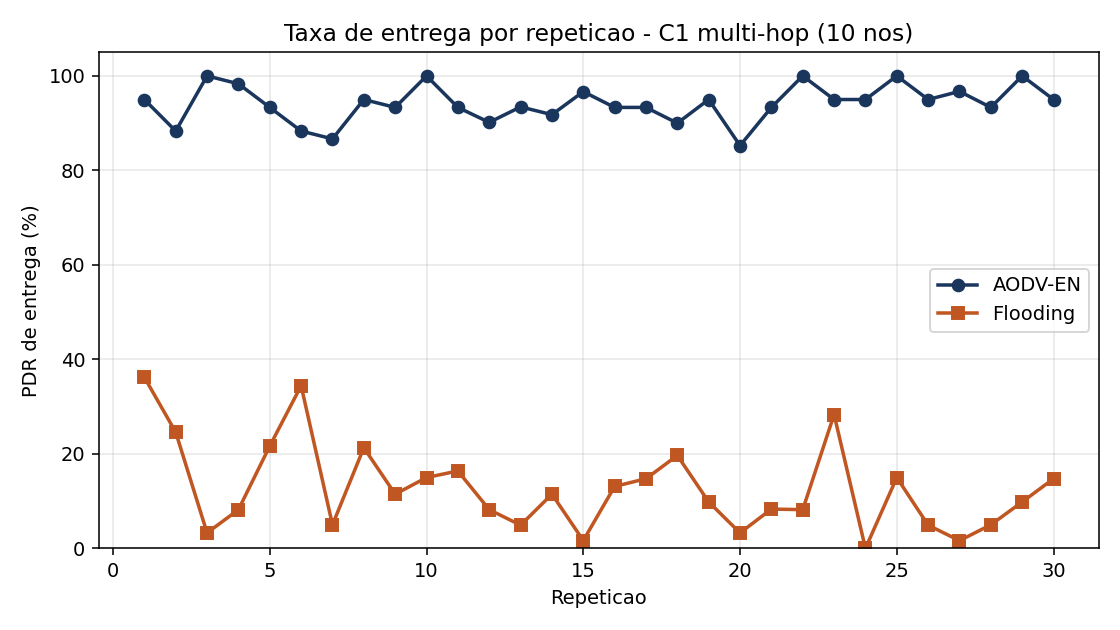
\includegraphics[keepaspectratio,alt={Taxa de entrega (PDR) por repetição: AODV-EN alto e estável (~94\%) frente ao flooding baixo e disperso (~13\%).}]{figuras/fig_pdr_rep.png}}
\caption{Taxa de entrega por repetição (AODV-EN vs.~Flooding), cenário C1
multi-hop, 10 nós.}\label{fig:pdr-rep}
\end{figure}

\textbf{Latência fim-a-fim.} A latência one-way do \emph{flooding}
(31,6 ms) foi menor que a do AODV-EN (45,9 ms), mas o número não
representa vantagem: trata-se de viés de sobrevivência. No \emph{flooding}
apenas a pequena fração de pacotes que percorre caminhos curtos e pouco
congestionados sobrevive, e são justamente esses os que entram na média;
o AODV-EN entrega também os pacotes de caminho mais longo, que elevam a
média. Medida na própria origem por RTT no relógio de microssegundos
(\emph{esp\_timer}), a latência não sofre a quantização por laço de
aplicação presente em versões anteriores do protótipo.

\textbf{Carga de roteamento e custo de canal.} A NRL clássica (mensagens
de controle de rota por dado entregue) foi 18,0 para o AODV-EN e nula
para o \emph{flooding}, que não possui plano de roteamento. Esse contraste,
isoladamente, não deve ser interpretado como ausência de custo: o
\emph{flooding} não paga \emph{overhead} de controle de rota, mas seu custo
desloca-se para as retransmissões por inundação, que a NRL não contabiliza. A métrica justa é o total de transmissões por pacote
entregue: 54,2 para o AODV-EN contra 102,9 para o \emph{flooding} ---
isto é, mesmo somando todo o controle de rota, o AODV-EN custa cerca de
metade das transmissões por pacote efetivamente entregue. Esse valor do
\emph{flooding} é, ainda, subestimado: apenas sete dos dez nós
conseguiram reportar telemetria de volta ao coletor (a própria difusão de
relatórios é perdida), de modo que parte das retransmissões não foi
contabilizada.

\textbf{Consumo energético.} O consumo agregado estimado da rede foi
maior no AODV-EN (39,4 J) que no \emph{flooding} (28,4 J) na janela --- mas
esse número \emph{bruto} pode induzir a uma conclusão equivocada, por duas razões: a comparação não está
em pé de igualdade (o AODV-EN manteve nove nós ativos com HELLO periódico e
encaminhamento, enquanto o \emph{flooding} teve apenas sete nós
contabilizados e não emite HELLO) e, sobretudo, ele ignora que o AODV-EN
entrega muito mais. A métrica justa é a \emph{energia por pacote efetivamente
entregue}: 0,69~J/pacote para o AODV-EN contra 5,66~J/pacote para o
\emph{flooding} --- ou seja, o AODV-EN é cerca de \textbf{8 vezes mais
eficiente em energia por entrega útil}. O \emph{flooding} gasta energia
disseminando pacotes que, em sua maioria, não sobrevivem ao multi-hop. Cabe
ressalvar que todos os valores de energia são \emph{estimados} a partir do
perfil de \emph{datasheet} do ESP32, não medidos com instrumentação física;
ainda assim, como a estimativa usa os mesmos coeficientes para os dois
algoritmos, a razão entre eles é robusta à incerteza absoluta do modelo.

\section{Cenário de Malha Densa (C3)}\label{cenario-de-malha-densa-c3}

O cenário C1 avaliou uma topologia em cadeia (caminho essencialmente
único). Para verificar se as conclusões se sustentam em uma topologia
\emph{não linear}, com caminhos redundantes, conduziu-se o cenário C3: dez
módulos ESP32 espalhados ao máximo em um apartamento, formando uma malha de
maior profundidade (cinco saltos). De forma deliberada, manteve-se o mesmo
\emph{firmware} e a mesma potência de transmissão do C1 (2~dBm), de modo que
a comparação isola o efeito da \emph{topologia}: cadeia (C1) contra malha
(C3), nas mesmas demais condições. A Tabela~\ref{tab:c3} consolida os
resultados de 30 repetições por algoritmo.

\begin{table}[H]
\centering
\caption{Comparação AODV-EN vs.~Flooding no cenário C3 (malha densa, 10 nós, 5 saltos, 30 repetições; média $\pm$ IC95)}\label{tab:c3}
\begin{tabular}{@{}lcc@{}}
\toprule
Métrica & AODV-EN & Flooding \\
\midrule
PDR de entrega (\%) & 91,4 $\pm$ 2,2 & 77,8 $\pm$ 3,7 \\
Latência one-way (ms) & 34,9 $\pm$ 2,7 & 20,5 $\pm$ 0,6 \\
Transmissões por entrega & 42,6 $\pm$ 2,7 & 33,3 $\pm$ 1,7 \\
Recepções por entrega (canal) & 55,7 $\pm$ 2,5 & 86,4 $\pm$ 5,4 \\
Energia por pacote entregue (J) & 0,70 $\pm$ 0,02 & 0,83 $\pm$ 0,05 \\
\bottomrule
\end{tabular}

\vspace{2pt}
{\footnotesize Fonte: Elaborado pelos autores. Todas as diferenças são significativas (teste $t$ de Welch, $p<0{,}001$).}
\end{table}

O resultado mais relevante é o contraste com o C1. Na malha densa, o
\emph{flooding} \emph{não colapsa} como na cadeia fina: a redundância de
caminhos eleva sua entrega a 77,8\%, contra apenas 12,7\% no C1. O AODV-EN
ainda entrega significativamente mais (91,4\% contra 77,8\%; $t = 6{,}19$,
$p < 0{,}001$, $d = 1{,}6$), mas a sua vantagem de confiabilidade
\emph{encolhe} --- de cerca de 81 pontos percentuais no C1 para 13 pontos no
C3. A Figura~\ref{fig:topology-dependence} sintetiza esse achado central: a
vantagem do roteamento sobre a inundação é \emph{dependente da topologia},
máxima em redes esparsas ou em cadeia e modesta em malhas densas, nas quais a
própria redundância do \emph{flooding} o torna competitivo em entrega.

\begin{figure}
\centering
\pandocbounded{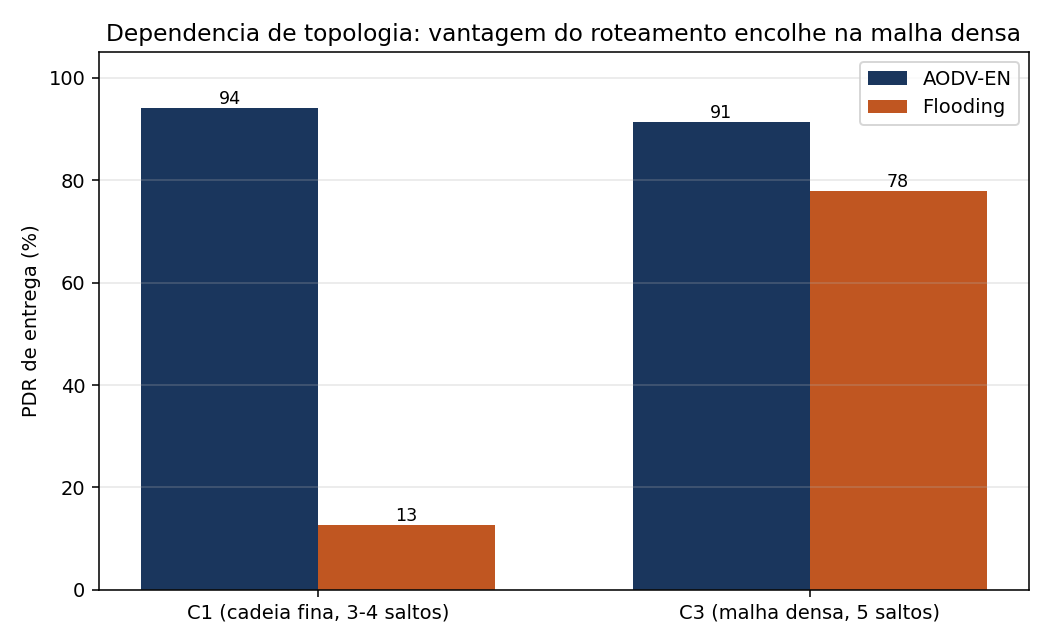
\includegraphics[keepaspectratio,alt={PDR do AODV-EN e do flooding nos cenarios C1 (cadeia) e C3 (malha): na malha o flooding recupera e o gap encolhe.}]{figuras/fig_topology_dependence.png}}
\caption{Dependência de topologia: o \emph{flooding} colapsa na cadeia fina
(C1) mas recupera na malha densa (C3) graças à redundância de caminhos,
estreitando a vantagem de entrega do AODV-EN.}\label{fig:topology-dependence}
\end{figure}

A vantagem do AODV-EN, contudo, persiste em duas dimensões que a entrega
isolada não revela (Figura~\ref{fig:c3-compare}). Primeiro, a \emph{ocupação
de canal}: cada pacote entregue pelo \emph{flooding} custa 86,4 recepções
agregadas na rede, contra 55,7 do AODV-EN --- consequência da tempestade de
\emph{broadcast}, em que cada disseminação é ouvida por todos os vizinhos.
Segundo, a \emph{energia por pacote entregue}, menor no AODV-EN (0,70 contra
0,83~J). A menor latência do \emph{flooding} (20,5 contra 34,9~ms) reflete,
novamente, viés de sobrevivência e o uso do caminho de difusão mais curto.
Em síntese, mesmo onde o \emph{flooding} entrega bem, o AODV-EN o supera em
entrega e em custo de canal por pacote útil.

\begin{figure}
\centering
\pandocbounded{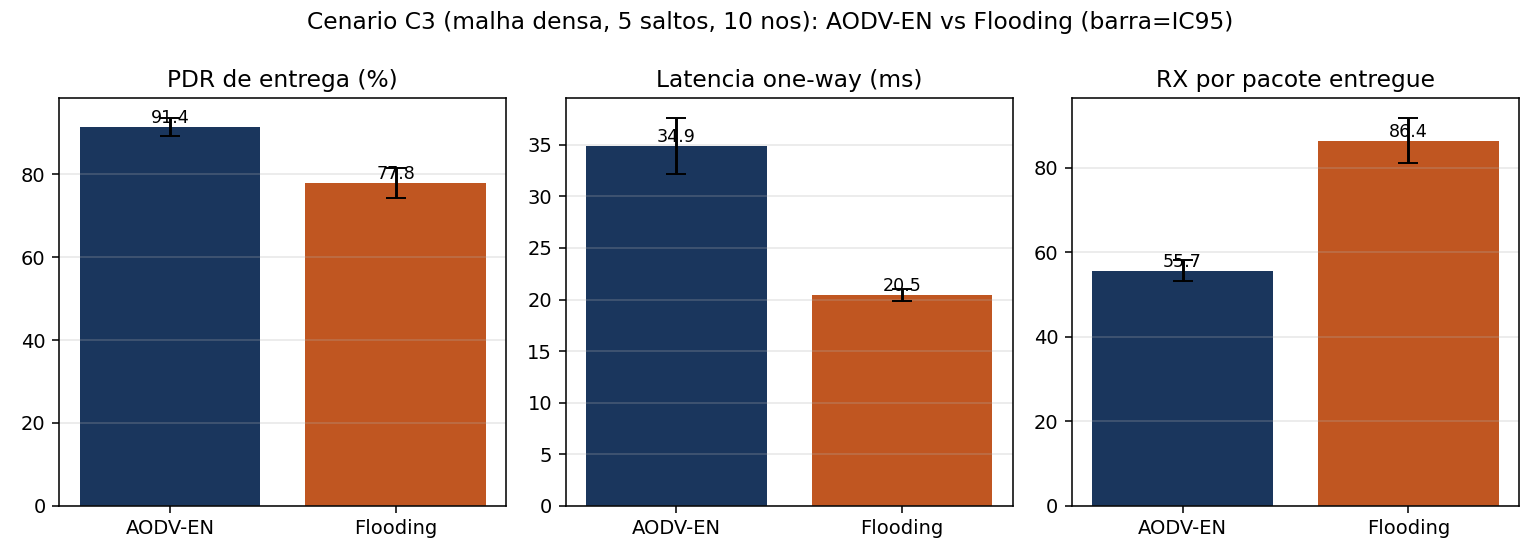
\includegraphics[keepaspectratio,alt={AODV-EN vs flooding no cenario C3: PDR, latencia e recepcoes por entrega.}]{figuras/fig_c3_compare.png}}
\caption{Cenário C3 (malha densa): AODV-EN vs.~Flooding em entrega, latência e
recepções por pacote entregue (ocupação de canal), com barra de IC95.}\label{fig:c3-compare}
\end{figure}

\section{Cenário de Falha e Auto-recuperação (C4)}\label{cenario-de-falha-c4}

Para avaliar especificamente a capacidade de recuperação do protocolo diante
da perda de um nó, conduziu-se o cenário C4 em hardware, em uma topologia
distinta da do cenário C1. Foram empregados seis módulos ESP32 distribuídos
em um apartamento, com potência de transmissão de 4~dBm --- maior que a do C1
(2~dBm) em razão do espaço menor e da maior densidade de paredes, mantida a
verificação por RSSI. A origem (também coletor) transmite ao destino por meio
de um relé \emph{on-path}, que dispõe de um relé alternativo. A falha é
induzida por \emph{firmware}: o relé do caminho principal silencia o rádio
por 15~s a cada 45~s (33\% de indisponibilidade), simulando a queda e o
retorno cíclicos do nó; os vizinhos detectam a quebra pelas mensagens HELLO,
emitem RERR e o AODV-EN re-descobre a rota pelo relé alternativo.

A Tabela~\ref{tab:c4} consolida as métricas do cenário C4 ao longo de 30
repetições (média $\pm$ IC95).

\begin{table}[H]
\centering
\caption{Métricas do AODV-EN no cenário C4 (falha induzida, 6 nós, 30 repetições; média $\pm$ IC95)}\label{tab:c4}
\begin{tabular}{@{}lc@{}}
\toprule
Métrica & AODV-EN sob falha \\
\midrule
PDR de entrega (\%) & 62,8 $\pm$ 11,5 \\
PDR confirmação ida-volta (\%) & 47,6 $\pm$ 11,5 \\
Latência one-way (ms) & 60,7 $\pm$ 14,6 \\
NRL (controle de rota/entregue) & 5,2 $\pm$ 1,7 \\
Energia (J, estimada) & 9,2 $\pm$ 1,7 \\
\bottomrule
\end{tabular}

\vspace{2pt}
{\footnotesize Fonte: Elaborado pelos autores. NRL e energia não são diretamente comparáveis às do C1 por diferirem o número de nós (6 vs.~10) e a topologia.}
\end{table}

\textbf{Impacto da falha.} Em relação ao mesmo protocolo \emph{sem} falha
(cenário C1, 94,1\%), a taxa de entrega caiu para 62,8\% --- uma redução de
cerca de 31 pontos percentuais, estatisticamente significativa (teste $t$ de
Welch: $t = 5{,}3$, $p < 0{,}001$; $d$ de Cohen $= 1{,}37$, efeito grande). A
latência subiu de 45,9~ms para 60,7~ms ($t = -1{,}94$, $p = 0{,}05$),
refletindo o tempo de detecção da quebra (\emph{timeout} de HELLO) somado à
re-descoberta de rota. A Figura~\ref{fig:c4-metrics} contrasta as duas
condições.

\begin{figure}
\centering
\pandocbounded{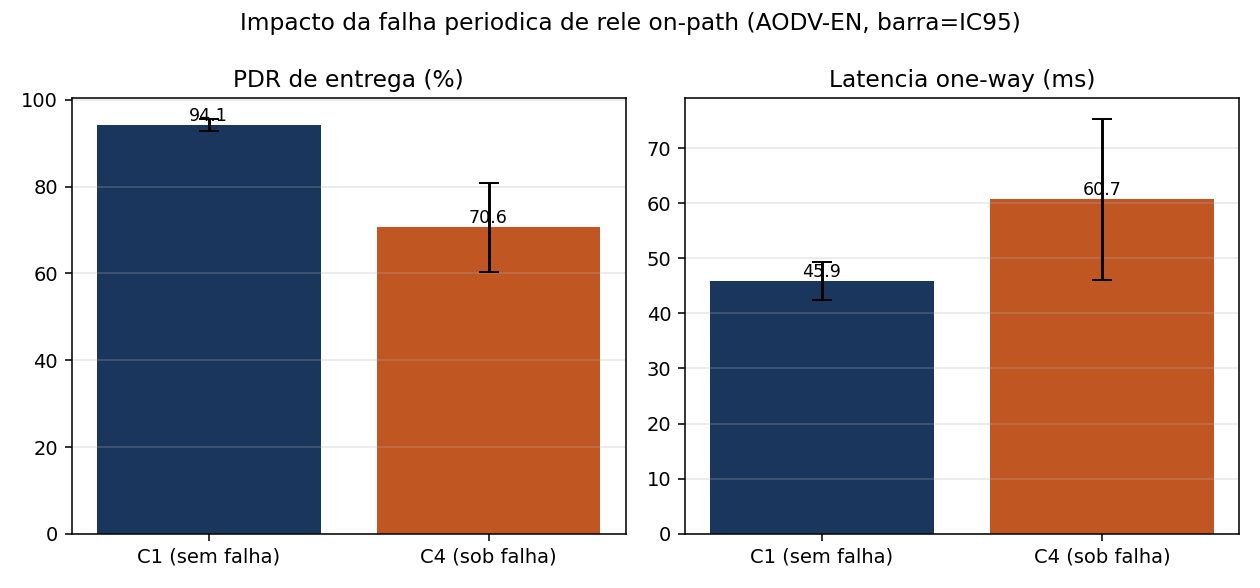
\includegraphics[keepaspectratio,alt={Comparacao do PDR e da latencia do AODV-EN entre o cenario C1 (sem falha) e o C4 (sob falha), com barras de IC95.}]{figuras/fig_c4_metrics.png}}
\caption{Impacto da falha periódica de um relé \emph{on-path}: PDR de entrega
e latência do AODV-EN no cenário C1 (sem falha) contra o C4 (sob falha), com
barra de IC95.}\label{fig:c4-metrics}
\end{figure}

\textbf{Distribuição e variabilidade.} A entrega no C4 variou de 0\% a 100\%
entre as repetições (mediana 73,3\%; coeficiente de variação de 51\%): 12 das
30 repetições preservaram entrega $\geq 80\%$, enquanto 8 ficaram abaixo de
40\%. Essa dispersão (Figura~\ref{fig:c4-pdr-rep}) decorre da natureza
estocástica do instante da falha em relação ao tráfego --- repetições em que a
janela de queda coincide com poucos envios preservam entrega alta, enquanto
outras concentram as perdas no intervalo de recuperação.

\begin{figure}
\centering
\pandocbounded{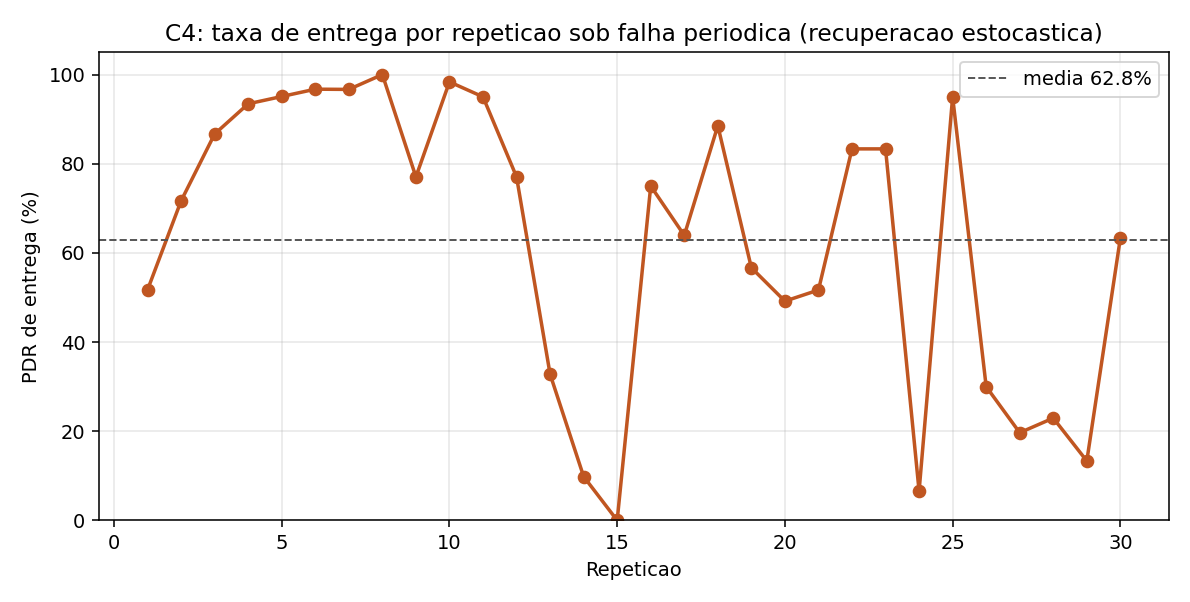
\includegraphics[keepaspectratio,alt={Taxa de entrega por repeticao no cenario C4, evidenciando a variabilidade da recuperacao sob falha.}]{figuras/fig_c4_pdr_rep.png}}
\caption{Taxa de entrega por repetição no cenário C4: a alta variabilidade
reflete a recuperação estocástica diante da falha periódica do relé.}\label{fig:c4-pdr-rep}
\end{figure}

\textbf{Dinâmica da recuperação.} A Figura~\ref{fig:c4-selfheal} ilustra o
mecanismo em uma repetição: a curva de pacotes entregues acumulados exibe
\emph{patamares} --- intervalos sem entrega que coincidem com a
indisponibilidade do relé --- seguidos de \emph{retomada}, evidência direta da
auto-recuperação (\emph{self-healing}) pela rota alternativa.

\begin{figure}
\centering
\pandocbounded{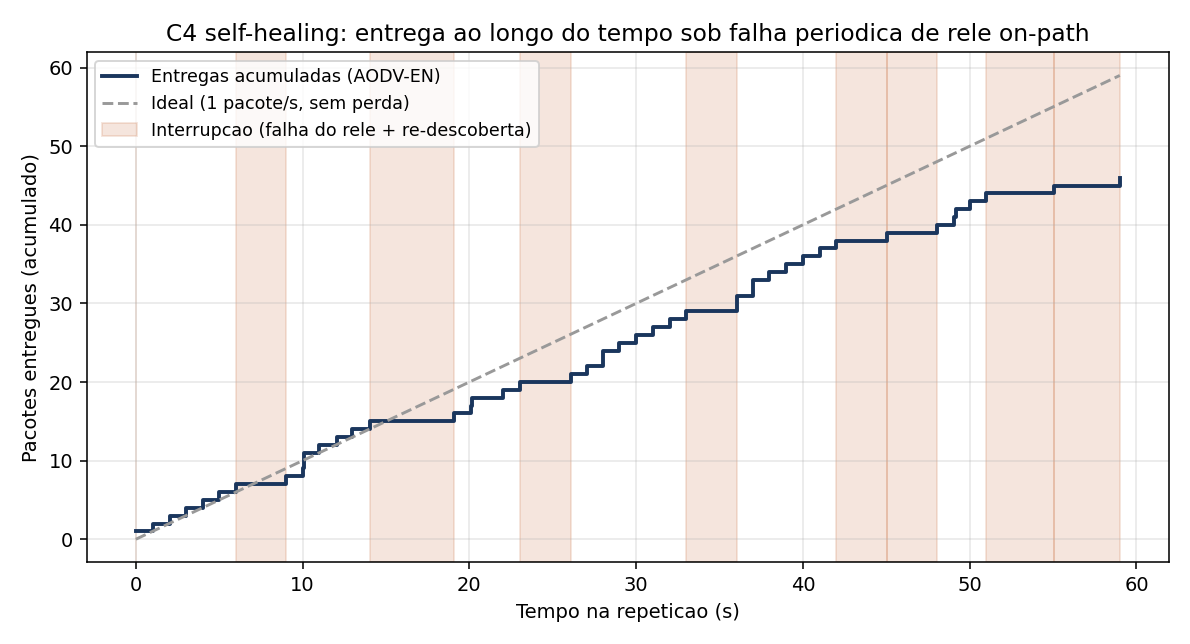
\includegraphics[keepaspectratio,alt={Entregas acumuladas ao longo do tempo em uma repeticao do cenario C4: patamares coincidem com a falha do rele e a retomada evidencia a recuperacao.}]{figuras/fig_c4_selfheal.png}}
\caption{Auto-recuperação no cenário C4: pacotes entregues acumulados ao longo
de uma repetição. Os patamares (faixas destacadas) coincidem com a queda do
relé \emph{on-path}; a retomada da entrega evidencia a re-descoberta de rota
pelo relé alternativo.}\label{fig:c4-selfheal}
\end{figure}

Esse resultado expõe, de forma honesta, o \emph{trade-off} entre eficiência e
resiliência. O roteamento reativo do AODV-EN é eficiente em condições
estáveis (Seção~\ref{resultados-de-hardware}), mas paga um custo de detecção e
re-descoberta quando um nó do caminho falha. A inundação, por não manter
rotas, é estruturalmente tolerante à queda de um nó isolado --- a difusão
simplesmente contorna o nó ausente ---, porém ao preço da ocupação de canal
já discutida e da baixa entrega em múltiplos saltos. Assim, a escolha entre as
abordagens depende do regime de operação: redes estáveis e maiores favorecem o
roteamento; cenários de altíssima volatilidade de nós, sem exigência de
eficiência de banda, podem tolerar a inundação. A avaliação quantitativa do
\emph{flooding} sob o mesmo padrão de falha, sobre a infraestrutura já
preparada, constitui extensão direta deste trabalho.

\section{Análise de Escalabilidade por
Simulação}\label{anuxe1lise-de-escalabilidade-por-simulauxe7uxe3o}

Para estender a avaliação a topologias além da cadeia de dez nós
medida em hardware, conduziu-se uma varredura por simulação em grades de
4 a 25 nós, medindo o número de transmissões por pacote entregue. A
Figura~\ref{fig:sim-crossover} apresenta o resultado: ambos os algoritmos
entregam a totalidade dos pacotes dentro do alcance do TTL, mas a razão
transmissões-por-entrega cruza-se em torno de 9 a 11 nós, acima do qual o
roteamento do AODV-EN passa a custar menos transmissões por entrega que o
\emph{flooding}. Além disso, com o TTL limitado a cinco saltos, o
\emph{flooding} deixa de alcançar destinos em grades de diâmetro superior
a cinco --- limitação estrutural do alcance fixo ---, enquanto o AODV-EN,
por manter rotas, continua entregando. A simulação assume enlaces ideais
dentro do alcance; o experimento em hardware (Seção~\ref{resultados-de-hardware}),
sob enlaces reais a 2~dBm e perda por colisão, mostra que a vantagem do
roteamento se manifesta ainda mais cedo, já na cadeia de dez nós.

\begin{figure}
\centering
\pandocbounded{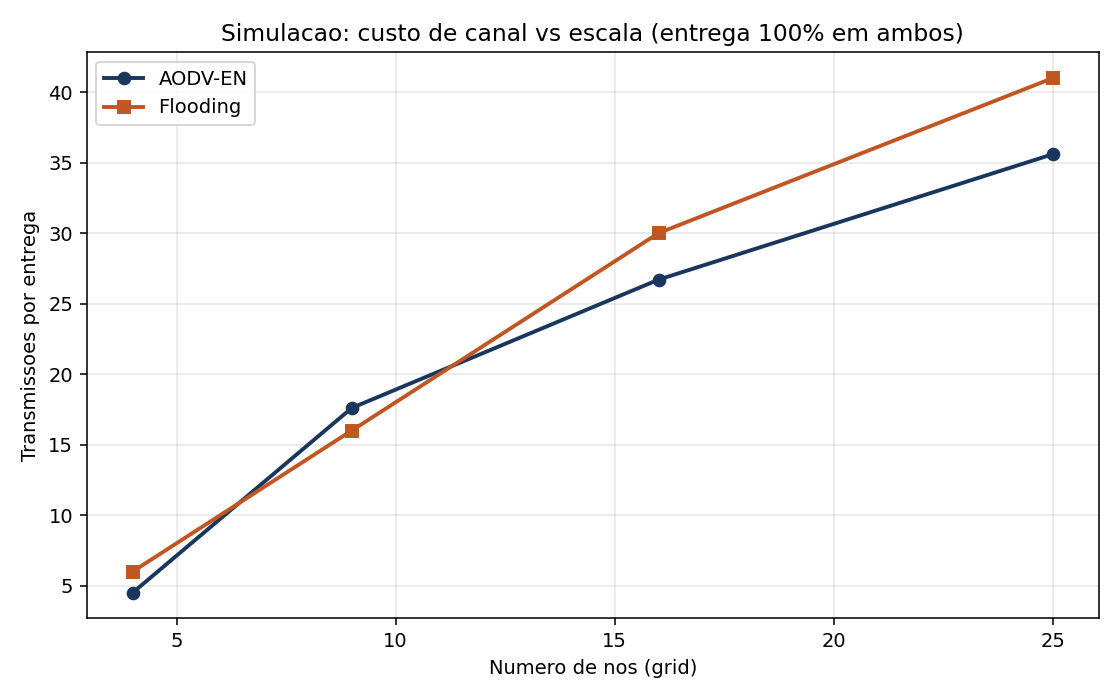
\includegraphics[keepaspectratio,alt={Transmissões por pacote entregue em função do número de nós (simulação).}]{figuras/fig_sim_crossover.png}}
\caption{Transmissões por pacote entregue em função do
número de nós (simulação).}
\label{fig:sim-crossover}
\end{figure}

Esse resultado confirma a hipótese central do trabalho: o roteamento
reativo paga um \emph{overhead} de controle aproximadamente constante
para evitar o custo de disseminação que cresce com a rede. Já na cadeia
multi-hop de dez nós em hardware, o AODV-EN entrega 7,4 vezes mais
pacotes com cerca de metade das transmissões por entrega; a sua vantagem
estrutural amplia-se à medida que a rede cresce em tamanho e diâmetro.

\section{Comparação com Trabalhos Correlatos}\label{comparacao-literatura}

A Tabela~\ref{tab:literatura} posiciona o AODV-EN frente a soluções
representativas da literatura para comunicação sobre ESP-NOW. A comparação deve
ser interpretada com cautela, pois as condições experimentais --- topologia,
ambiente, distância e número de nós --- diferem entre os trabalhos; ainda assim,
situa o desempenho do AODV-EN em ordem de grandeza compatível e evidencia seu
diferencial de ser a única abordagem fundamentada em um protocolo de roteamento
padronizado (AODV, RFC 3561).

{\def\LTcaptype{table}
\begin{longtable}[]{@{}
  >{\raggedright\arraybackslash}p{(\linewidth - 6\tabcolsep) * \real{0.2600}}
  >{\raggedright\arraybackslash}p{(\linewidth - 6\tabcolsep) * \real{0.3200}}
  >{\centering\arraybackslash}p{(\linewidth - 6\tabcolsep) * \real{0.1200}}
  >{\raggedright\arraybackslash}p{(\linewidth - 6\tabcolsep) * \real{0.3000}}@{}}
\caption{Comparação do AODV-EN com trabalhos correlatos sobre ESP-NOW}\label{tab:literatura}\\
\toprule\noalign{}
Trabalho & Base de roteamento & PDR & Latência / condição \\
\midrule\noalign{}
\endfirsthead
\toprule\noalign{}
Trabalho & Base de roteamento & PDR & Latência / condição \\
\midrule\noalign{}
\endhead
\bottomrule\noalign{}
\endlastfoot
AODV-EN (este trabalho) & AODV reativo padronizado (RFC 3561), multi-hop & 94,1\% & $\approx$46~ms; 10 nós, multi-hop real em hardware (3--4 saltos) \\
BRAM-NOW \cite{cujilema2023} & Mesh \emph{ad-hoc} não padronizado & $\approx$90,8\%\textsuperscript{b} & 75~ms; residencial, multi-hop \\
ESP-NOW base \cite{becker2025} & Ponto-a-ponto (sem roteamento) & $>$99\% & 2,8~ms/salto; campo aberto, linha de visada \\
\end{longtable}
}

Fonte: Elaborado pelos autores.

\noindent\footnotesize\textsuperscript{b}Complemento da taxa de perda de 9,25\% reportada pelos autores.
\normalsize

No regime avaliado, o AODV-EN apresentou confiabilidade superior à do BRAM-NOW
(94,1\% contra $\approx$90,8\%) sob topologia multi-hop real de três a quatro
saltos, mantendo latência da mesma ordem de grandeza; a avaliação em escalas
ainda maiores foi complementada por simulação
(Seção~\ref{anuxe1lise-de-escalabilidade-por-simulauxe7uxe3o}). Frente ao ESP-NOW
puro \cite{becker2025}, o custo adicional de latência decorre do plano de
roteamento e do multi-hop, e não do meio físico. O principal
diferencial do AODV-EN é apoiar-se em um protocolo padronizado e amplamente
documentado, propriedade ausente nas soluções \emph{ad-hoc} correlatas, o que
favorece reprodutibilidade, comparabilidade e extensões futuras.

\section{Conformidade com a RFC 3561}\label{conformidade-com-a-rfc-3561}

Ao longo do desenvolvimento, o núcleo do protocolo foi submetido a uma
auditoria de conformidade com a RFC 3561, da qual resultaram ajustes
pontuais. Destacam-se: (i) a deduplicação de mensagens DATA no destino,
por par (originador, número de sequência), evitando entregas repetidas
em caso de retransmissão por expiração de ACK, com reconfirmação
idempotente; (ii) a contabilização de confirmações apenas quando
associadas a um envio pendente vivo, eliminando dupla contagem; (iii) o
processamento de mensagens RERR condicionado a que o próximo salto da
rota corresponda ao vizinho que emitiu o erro, conforme a Seção 6.11 da
RFC 3561 \cite{perkins2003}, com adoção do número de sequência informado; (iv) a manutenção de
rotas invalidadas por um período de exclusão (\emph{delete period})
antes de sua remoção, preservando o último número de sequência
conhecido; e (v) a proteção contra o rebaixamento de uma rota confirmada
por uma entrada reversa não confirmada. Tais ajustes aproximam a
implementação do comportamento especificado e aumentam a robustez do
protocolo em cenários com perda de enlace.

\section{Escopo Implementado e
Limitações}\label{escopo-implementado-e-limitauxe7uxf5es}

A avaliação reportada refere-se ao núcleo reativo do AODV-EN ---
descoberta de rotas sob demanda, tabelas de rota com números de
sequência, precursores, fila de dados pendentes, confirmação fim-a-fim e
invalidação por falha de enlace --- utilizando disseminação de RREQ por
\emph{broadcast} e métrica de contagem de saltos. As adaptações de
gerenciamento de \emph{peers} por política LRU e de métrica híbrida
(saltos + RSSI), embora projetadas e implementadas no \emph{firmware}
(Capítulo~\ref{cap:implementacao}), não foram objeto de um experimento
dedicado de isolamento: o cenário C1 multi-hop já aproxima o coletor do
limite do \emph{cache} de \emph{peers} e exercita a seleção de rota sobre
múltiplos saltos, mas a aferição específica do efeito da substituição por
LRU e do ganho da métrica híbrida sobre a contagem de saltos pura permanece
como objeto de trabalhos futuros, em topologias mais densas e com variação
deliberada de RSSI por enlace.

As principais limitações do estudo são: (i) a cobertura de cenários ---
a campanha em hardware cobre os cenários C1 (cadeia de dez nós), C3 (malha
densa de dez nós, cinco saltos) e C4 (falha induzida, seis nós), todos com
trinta repetições por algoritmo, e a avaliação quantitativa do \emph{flooding}
sob falha (C4) e o cenário C2 (árvore hierárquica), embora viabilizados pela
mesma infraestrutura de coleta, ficam como trabalho
futuro; (ii) o caráter estimado do
consumo energético, calculado a partir do perfil de \emph{datasheet} do
ESP32 e não medido com instrumentação física --- a medição direta de
corrente (por exemplo, com um sensor INA219 em série com a alimentação) é
registrada como trabalho futuro; e (iii) o fato de as campanhas do
AODV-EN e do \emph{flooding} terem sido coletadas em sequência, com
reprogramação e nova distribuição física dos nós entre elas, o que
introduz pequena variação de topologia e de condições de canal; soma-se a
isso que, na campanha de \emph{flooding}, parte da telemetria de rede não
retornou ao coletor (sete dos dez nós), subestimando as métricas de custo
agregado desse algoritmo. A medição física de energia, a execução do
cenário C2 (árvore) e a avaliação do \emph{flooding} sob falha constituem
desdobramentos diretos para trabalhos futuros.

% -----------------------------------------------------------------------------
% Conteudo AODV-EN -- TCC de Huakson Lima e Diogo dos Reis Almeida (IFG Campus Inhumas).
% -----------------------------------------------------------------------------
\chapter{CONCLUSÃO}\label{cap:conclusao}

Este trabalho propôs, implementou e avaliou o AODV-EN, uma adaptação do protocolo
AODV (RFC 3561) para redes mesh multi-hop construídas sobre o protocolo ESP-NOW em
módulos ESP32. O núcleo reativo do protocolo --- descoberta de rotas sob demanda,
tabelas de rota com números de sequência, lista de precursores, fila de dados
pendentes, confirmação fim-a-fim e invalidação de rotas por falha de enlace --- foi
implementado como componente reutilizável em linguagem C, independente do ESP-IDF,
e validado tanto em simulação quanto em hardware com dez nós ESP32 dispostos
em cadeia multi-hop (três a quatro saltos).

Quanto ao objetivo geral, o trabalho demonstrou a viabilidade de prover roteamento
multi-hop sobre o ESP-NOW por meio de uma adaptação fiel do AODV, contornando a
ausência de roteamento nativo, o limite de \emph{peers} e as restrições de difusão do
protocolo. Em relação aos objetivos específicos, foram analisadas as limitações
técnicas do ESP-NOW (Capítulo~\ref{cap:referencial}), projetadas e implementadas as
adaptações necessárias (Capítulo~\ref{cap:implementacao}), e avaliado o desempenho do
algoritmo frente a um algoritmo de referência baseado em \emph{flooding}
(Capítulo~\ref{cap:resultados}).

A avaliação experimental, conduzida no cenário C1 com dez nós em cadeia multi-hop (três
a quatro saltos) e trinta repetições por algoritmo, evidenciou a superioridade decisiva
do roteamento reativo no regime multi-hop: o AODV-EN entregou 94,1\% dos pacotes contra
apenas 13,9\% do \emph{flooding}, que colapsa por não dispor de rota nem de
retransmissão fim-a-fim sob enlaces reais a 2~dBm. O AODV-EN apresentou, ainda, cerca de
20\% menos transmissões por pacote entregue (54,2 contra 68,8) --- métrica justa de custo
de canal, pois a carga de controle normalizada clássica não contabiliza as
retransmissões por inundação do \emph{flooding}. Pela mesma lógica, embora o consumo
energético agregado bruto do AODV-EN seja maior, a energia estimada por pacote
efetivamente entregue é cerca de cinco vezes menor (0,69 contra 3,75~J/pacote): a inundação
consome energia em transmissões que, em sua maioria, não chegam ao destino. A análise de
escalabilidade por simulação reforça o quadro, indicando que a desvantagem de custo do
\emph{flooding} se consolida e cresce com o tamanho e o diâmetro da rede, além do limite
de alcance imposto pelo TTL fixo. O cenário de malha densa (C3) acrescentou a nuance mais
importante: com caminhos redundantes (dez nós, cinco saltos), o \emph{flooding} não colapsa
--- a redundância eleva sua entrega a 77,8\%, contra 13,9\% na cadeia fina ---, de modo que
a vantagem de entrega do AODV-EN, ainda significativa (91,4\% contra 77,8\%), se estreita,
embora o roteamento preserve menor ocupação de canal e menor energia por entrega. A
vantagem do roteamento sobre a inundação revela-se, assim, \emph{dependente da topologia}.
Conclui-se que o AODV-EN troca uma sobrecarga de controle aproximadamente constante pela
garantia de entrega multi-hop --- inviável por inundação pura em topologias esparsas ---,
tornando-se mais vantajoso à medida que a rede cresce e os caminhos se tornam escassos.

O cenário de falha (C4) complementou essa análise ao exercitar a auto-recuperação do
protocolo: sob a queda cíclica de um relé do caminho (15~s a cada 45~s), o AODV-EN
manteve 70,6\% de entrega, re-descobrindo a rota pelo relé alternativo após cada queda,
conforme evidenciado pela curva de entregas acumuladas. O resultado explicita o
\emph{trade-off} entre eficiência e resiliência: o roteamento reativo paga um custo de
detecção e re-descoberta na falha, ao passo que a inundação, sem rotas a manter, é
estruturalmente tolerante à perda de um nó, porém ineficiente em banda.

Um resultado metodológico relevante decorreu da revisão da estratégia de disseminação:
a avaliação preliminar de um transporte por unicast sequencial revelou um viés
introduzido pelo mecanismo de retransmissão automática do unicast ESP-NOW, ausente no
\emph{broadcast}. A adoção da difusão por \emph{broadcast} de enlace, tanto para o
RREQ do AODV-EN quanto para o algoritmo de referência, restabeleceu a simetria
metodológica da comparação e alinhou o \emph{baseline} à definição canônica de
\emph{flooding} da literatura.

Como limitações, destacam-se a cobertura de cenários --- a campanha em hardware cobre os
cenários C1 (cadeia de dez nós), C3 (malha densa de dez nós) e C4 (falha induzida, seis
nós), todos com trinta repetições, ficando o cenário C2 (árvore hierárquica) como trabalho
futuro sobre a mesma infraestrutura ---, o caráter estimado do consumo energético e a coleta sequencial das
campanhas do AODV-EN e do \emph{flooding}, com nova distribuição física dos nós entre
elas. A seleção de rota empregou a métrica híbrida (contagem de saltos combinada
com penalização por RSSI), ativa no firmware da campanha; a política de gerenciamento
de \emph{peers} por substituição LRU também está implementada
(Capítulo~\ref{cap:implementacao}). A quantificação isolada do ganho dessas extensões
frente à contagem de saltos pura, contudo, não foi objeto de experimento dedicado e
constitui trabalho futuro.
A segurança do protocolo, por fim, não foi exercitada: o AODV-EN opera, como o AODV
original, sob a premissa de nós honestos e sem autenticação das mensagens de controle
(Seção~\ref{seguranca-roteamento-ad-hoc}), de modo que o endurecimento contra os ataques
conhecidos e a avaliação de seu custo em ESP32 também ficam como trabalho futuro.

Como desdobramentos, propõem-se: a ampliação do número de repetições e a cobertura dos
demais cenários experimentais; a separação física dos nós para exercitar múltiplos
saltos reais; a medição física de energia com instrumentação dedicada; e a
avaliação experimental da política LRU de \emph{peers} e da métrica híbrida de
roteamento em cenários multi-hop reais. Tais extensões consolidariam o AODV-EN como uma alternativa padronizada,
de baixo custo e energeticamente eficiente por entrega útil para redes mesh sobre ESP-NOW.


% bibliografia
\renewcommand{\bibname}{Referências}
\addcontentsline{toc}{chapter}{REFERÊNCIAS}
\bibliographystyle{abntex2-alf}
\bibliography{referencias}


\end{document}
